\chapter{Functional connectivity hubs of the mouse brain}

\label{Chapter02}

\begin{quote}
    This chapter has been published as:

    \longfullcite{liska2015}
\end{quote}

%------------------------------------------------------------------------------
%	SECTION 1
%------------------------------------------------------------------------------
\section{Background} 
Resting-state BOLD functional magnetic resonance imaging (rsfMRI) has been
widely employed to investigate the intrinsic functional organization of the
human brain \parencite{bullmore2009}. Graph theory representations of rsfMRI
networks, whereby brain connectivity is conceptualized as a set of nodes
(neuronal elements) and edges (their interconnections), have demonstrated that
the human brain has topological features recapitulating the defining
characteristics of complex networks \parencite{watts1998}, including the
presence of functionally specialised modules encompassing well-characterized
neurofunctional systems \parencite{fair2009, meunier2009, power2011}. In order
to account for the brain’s ability to simultaneously coordinate multiple
networks systems and ensure efficient communication, the presence of functional
hub nodes serving as integrators of distinct neuronal systems has been
hypothesized. Numerous rsfMRI studies have indicated the presence of
highly-connected cortical regions as putative functional hubs for the human
brain, most of which appear to exhibit overlap with sub-regions of the default
mode network (DMN) \parencite{cole2010, tomasi2011, zuo2012}. Importantly, the
integrative role of these hub regions renders them points of potential
vulnerability to dysfunction in brain disorders. Consistent with this notion,
aberrant rsfMRI connectivity profiles have been described for several hub
regions in pathological conditions such as autism, schizophrenia and
neurodegenerative disorders \parencite{buckner2009, vandenheuvel2013}. However,
fundamental issues related to the etiopathological and biological foundations of
these alterations remain to be addressed. For one, the neurophysiological
cellular underpinnings of functional hub derangement observed in
neuropsychiatric disorders remain largely unknown.  It is also unclear whether
these alterations are patho-physiologically relevant, or just epiphenomenal to
underlying brain disorders.

Functional hub identification in preclinical species like the mouse, where
genetic, cellular and molecular underpinnings of several brain disorders can be
reproduced in controlled conditions and manipulated with cellular specificity
\parencite{deisseroth2011}, may offer new critical insight into the
above-mentioned issues. Initial attempts to unravel the rodent’s brain
functional topology have been carried out in rats \parencite{dsouza2014,
liang2011, liang2012} and more recently in mice \parencite{mechling2014,
stafford2014}. By using independent-component analysis (ICA) decomposition of
rsfMRI signals in awake rats, \textcite{liang2011} reported the
presence of three large modules, covering cortical areas, prefrontal and limbic
hippocampal regions and basal forebrain structures, respectively. Using
anatomically-defined labels, \textcite{dsouza2014} identified six
communities in medetomidine sedates rats, including two purely cortical systems
(i.e. frontal and somatosensory) together with four mixed communities involving
hippocampal and peri-hippocampal cortices, basal ganglia, thalamic nuclei and
pons. ICA-based decomposition has also been recently applied to mouse rsfMRI
datasets acquired under isoflurane anaesthesia \parencite{mechling2014}, leading
to the identification of a basal ganglia module plus four other composite
communities which included complex combinations of cortical and subcortical
systems. Two of the above studies also report attempts to identify
inter-connecting hub regions. \textcite{dsouza2014} attributed a putative
integrative function to the hippocampus, striatum plus all cortical subdivision,
with the sole exception of visual, primary motor and parietal cortices. These
latter regions are part of a set of eleven putative hub regions described by
\textcite{mechling2014} in the mouse brain, which also included somatosensory,
frontal as well as subcortical diencephalic structures and the striatum.
Collectively, while these initial studies led to the identification of seemingly
stable functional partitions, substantial heterogeneity exists in their
anatomical composition, as well as in the location of integrative structures, a
finding that may reflect discrepant experimental procedures (e.g. anaesthesia,
preprocessing procedures) and is probably exacerbated by heterogeneity in the
regional parcellation schemes (coarse ICA-based, or anatomical volumes) and
network thresholding strategies employed. Moreover, none of the functional
partitions described so far can be straightforwardly related to known
distributed human networks (e.g.  DMN), which is a limiting factor in the
translation of preclinical research to human condition. 

Employing rigorous control of motion and potential physiological confounds
\parencite{ferrari2012}, we recently demonstrated the presence of robust
distributed rsfMRI networks in the mouse brain \parencite{zhan2014}, including
functional precursors of the human salience and default mode networks
\parencite{sforazzini2014, sforazzini2016}, an observation recently replicated
by an independent group \parencite{stafford2014}. Our datasets offer the
opportunity to spatially locate functional hubs in the mouse brain and relate
them to known network system of the human brain, which greatly enhances the
translational value of this approach. To this purpose, here we applied a
computationally unbiased, fully-weighted network analysis of rsfMRI connectivity
at a voxel scale in a large cohort of adult mice. We show the presence of six
large-scale functional partitions, and anatomically localise mutually
inter-connected hubs in several sub-regions of the DMN as well as in several
cortical association areas of the mouse brain. These bear a strong resemblance
to findings in the human brain, suggesting the presence of evolutionarily
conserved cortical regions serving as integrators of segregated brain systems in
the mouse, and supporting the use of this species to investigate aberrant rsfMRI
hub connectivity associated to brain pathological states.

\section{Materials and methods}
ll in vivo studies were conducted in accordance with the Italian law (DL 116,
1992 Ministero della Sanità, Roma) and the recommendations in the Guide for the
Care and Use of Laboratory Animals of the National Institutes of Health. Animal
research protocols were also reviewed and consented to by the animal care
committee of the Istituto Italiano di Tecnologia (permit 07-2012). All surgical
procedures were performed under anaesthesia.

\subsection{Animal preparation}
MRI experiments were performed on male 20-24 week old C57BL/6J (B6) mice (n=41,
Charles River, Como, Italy). The animal preparation protocol was recently
described in detail \parencite{ferrari2012, sforazzini2014, sforazzini2016,
zhan2014}.  Briefly, mice were anaesthetized with isoflurane (5\% induction),
intubated and artificially ventilated (2\% maintenance). The left femoral artery
was cannulated for continuous blood pressure monitoring and blood sampling. At
the end of surgery, isoflurane was discontinued and substituted with halothane
(0.75\%).  Functional data acquisition commenced 45 min after isoflurane
cessation. Mean arterial blood pressure was recorded throughout the imaging
sessions. Arterial blood gases (paCO2 and paO2) were measured at the end of the
functional time series to exclude non physiological conditions. Mean paCO2 and
paO2 levels recorded were $20\pm5$ and $257\pm33$ mmHg, respectively, well
within the physiological range.  

\subsection{Image data acquisition}
All in vivo experiments were performed using a 7.0 Tesla MRI scanner (Bruker
Biospin, Milan). Transmission and reception were achieved using a 72 mm birdcage
transmit coil and a custom-built saddle-shaped four-channel solenoid coil for
signal reception. Shimming was performed on a 6mm $\times$ 6mm $\times$ 6mm
region, using a FASTMAP protocol. For each session, high-resolution anatomical
images were acquired with a fast spin echo sequence (RARE, hennig1986) with the
following parameters: repetition time (TR)/echo time (TE) 5500/60 ms, matrix 192
$\times$ 192, field of view 2 $\times$ 2 $\text{cm}^2$, 24 coronal slices, slice
thickness 0.50 mm. Co-centred single-shot BOLD rsfMRI time series were acquired
using an echo planar imaging (EPI) sequence with the following parameters: TR/TE
1200/15 ms, flip angle $30\degree$, matrix 100 $\times$ 100, field of view 2
$\times$ 2 $\text{cm}^2$, 24 coronal slices, slice thickness 0.50 mm, 300
volumes and a total rsfMRI acquisition time of 6 min.

\subsection{Image data preprocessing}
Image preprocessing was carried out using tools from FMRIB Software Library
(FSL, v5.0.6; \url{http://fsl.fmrib.ox.ac.uk/fsl/}) \parencite{jenkinson2012}
and AFNI (v2011\_12\_21\_1014; \url{http://afni.nimh.nih.gov/afni/}). RsfMRI
time series were despiked (AFNI/3dDespike), corrected for motion
(AFNI/3dvolreg), and spatially normalized to an in-house C57Bl/6J mouse brain
template \parencite{sforazzini2016} (FSL/FLIRT, 12 degrees of freedom). The
normalized data had a spatial resolution of 0.2 $\times$ 0.2 $\times$ 0.5
$\text{mm}^3$ (99 $\times$ 99 $\times$ 24 matrix). Head motion traces and mean
ventricular signal (averaged fMRI time course within a manually-drawn ventricle
mask) were regressed out of each of the time series (AFNI/3dDeconvolve). To
assess the effect of global signal removal, separate rsfMRI time series with the
whole-brain average time course regressed out were also generated. All rsfMRI
time series were spatially smoothed (AFNI/3dmerge, Gaussian kernel of full width
at half maximum of 0.5 mm) and band-pass filtered to a frequency window of
0.01-0.08 Hz (AFNI/3dBandpass) \parencite{sforazzini2016}.

\subsection{Functional network formation}
Time courses from all voxels in a brain tissue mask associated with the
anatomical template  were extracted and a 16135 $\times$ 16135 connectivity
matrix was calculated for each subject using Pearson product-moment correlation
coefficient as a measure of inter-voxel connectivity \parencite{bullmore2009},
resulting in subject-wise functional connectivity networks. In contrast to the
vast majority of network analyses of rsfMRI data, the connectivity matrix was
not subject to any further arbitrary thresholding and/or binarisation
\parencite{bullmore2009}. Separate connectivity matrices were created for the
rsfMRI dataset with global signal regression.

\subsection{Module detection}
Most of network attributes used to identify functional hubs rely on a prior
detection of modules that accurately describe the topological organization of
brain networks \parencite{sporns2013}. To this purpose, standard approaches in
human and rodent brain analyses employ a modular partition based on a
connectivity network averaged across a large number of subjects
\parencite{dsouza2014, liang2011, liang2012, mechling2014, power2011, power2013,
rubinov2010, yeo2011,  zuo2012}. Accordingly, the subject-wise connectivity
matrices were first transformed to z scores using Fisher’s r-to-z transform,
averaged across all animals and transformed back to r values to create the
average functional network. 

The average functional network was then partitioned into non-overlapping modules
by maximizing the modularity of the final partition \parencite{newman2004} using
the Louvain algorithm \parencite{blondel2008}, as implemented in Brain
Connectivity Toolbox (BCT) \parencite{rubinov2010}. An asymmetric measure of
modularity incorporating both positive and negative weights was employed
\parencite{rubinov2011}. Corresponding average null networks, against which we
compared the resulting modularity value \parencite{guimera2004}, were created
from subject-wise null networks, each matching the covariance structure of a
single subject connectivity matrix \parencite{zalesky2012}.

The robustness of the resulting modules was further assessed by taking advantage
of the non-deterministic nature of the Louvain algorithm \parencite{blondel2008}
and investigating the presence of competing maxima, whose presence is suggestive
of an absence of a clear modular structure \parencite{gfeller2005, karrer2008,
massen2006, wilkinson2004}. To this purpose, we performed 100 independent
iterations of the algorithm, each with a randomized order of nodes on input, and
created iteration stability maps of modules by calculating for each node the
proportion of iterations in which it was assigned to each module. These
iterations yielded a consistent output and, as further analyses required one
single modular structure, a reference partition of the mouse functional network
was created by assigning each voxel to the module to which it belonged in more
than 50 \% of iterations. This procedure was carried out on rsfMRI datasets with
and without global signal regression. 

The two cortical modules identified in our study, the default mode network (DMN)
and lateral cortical network (LCN), have been previously shown to be
anticorrelated in both mice and rats \parencite{schwarz2013a, sforazzini2016}.
To investigate the presence of analogous anticorrelations in the present dataset
upon global signal regression, we extracted the mean signals from the identified
cortical modules and correlated them with all voxels within the brain to obtain
T statistics maps.

To assess inter-subject variability of the modular structure, subject-wise
connectivity matrices were partitioned using the same method and the similarity
of each pair of individual partitions was quantified with the variation of
information (VI) metric \parencite{rubinov2011}, achieving a mean VI value of 0.2412 ($\sigma =
0.0203$). The same procedure was repeated for subject-wise null networks,
constructed as described above, achieving a mean VI value of 0.2889 ($\sigma =
0.0116$). A paired t-test between the corresponding VI values confirmed that the
level of reproducibility is highly statistically significant ($p < 0.00001$).
Moreover, the effect size obtained (2.9) was of similar order of magnitude to a
recent rat study \parencite{dsouza2014}.

In order to assess the impact of spatial smoothing and voxel ''adjacency'' on
the detection of functional modules \parencite{power2011}, we created two
additional functional networks in which we removed connections shorter than 0.5
mm and 1.0 mm, respectively. We then separately identified modules in these two
additional networks for comparisons with original functional partitions.

\subsection{Global and module hub identification}
Functional hubs have commonly been defined as nodes with a high density of
connections across the whole network \parencite{bullmore2009}. However,
consideration of node connectivity distributions within and between the
different component modules allows a more nuanced view of topological function
and node roles within the overall network \parencite{guimera2005,
vandenheuvel2013, zuo2012}. In particular, it allows candidate hubs to be
defined based on high connectivity within the overall network, within their own
module and to nodes in other modules.

Normalized positive connection strength of a node in a weighted network (also
referred to as strength) quantifies the overall density of its connections
across the whole network and is defined as the sum of all positive connections
of the node:

$$s_i =  \frac{\sum_{w_{ij}>0} w_{ij}}{N-1},$$
where $w_{ij}$ is the weight of the connection between nodes $i$ and $j$, and
$N$ is the number of nodes in the network \parencite{rubinov2011}.

Conversely, connection diversity of a node assesses the distribution of its
connections across modules, i.e., whether the node preferentially connects only
to a limited subset of modules (low diversity) or whether its connections are
spread evenly across the whole network (high diversity) \parencite{rubinov2011}.
The values of connection diversity are in the range of $[0,1]$ and the measure
is formally defined as:

$$h_i = - \frac{1}{\log M} s_i(u) \log{s_i(u)},$$
where $M$ is the number of modules and $s_i(u)$ is the strength of node $i$
within module $u$. The diversity parameter captures, for complete weighted
networks, topological functionality analogous to the participation coefficient
in binary networks \parencite{guimera2005}.

The strength of node $i$ within module $u$ is defined as: 

$$s_i(u) = \frac{\sum_{w_{ij}>0} w_{ij} \delta_u(j)}{N-1},$$
where $\delta_u (j)=1$ when $j$ is part of module $u$, and $\delta_u(j) = 0$
otherwise (i.e., only connections of node $i$ to nodes $j$ within module $u$
contribute to the summation) \parencite{rubinov2011}. Within this framework, we
refer to the strength of a node within its own module as the within-module
strength of the node. 

\textcite{guimera2005} elaborated a number of node roles in a
''functional cartography'' of the within- vs. between-module connectivity
landscape of binary networks. While this presents an appealing conceptual
framework, the proposed definitions were based on somewhat arbitrary (although
intuitive) divisions of the parameter space. Analogous parameter-space divisions
for fully weighted networks of functional connectivity have yet to be defined,
and should meaningfully reflect both the network characteristics and underlying
biology. A critical first step in elucidating the connectivity landscape of
these neurobiological networks is to localise and understand the behaviour of
the extreme nodes, i.e. those with maximal connection strength or diversity. 

To identify and characterise extreme nodes, we implemented the statistical ''top
percentage'' threshold approach \parencite{cole2010}, which identifies the
highest strength and diversity regions and at the same time quantifies
inter-subject consistency and avoids arbitrary strength or diversity
thresholding. Briefly, this approach consists in calculating connection
strength, connection diversity and within-module strength maps separately for
each subject, converting them to standard scores and performing a series of
one-tailed one-sample t-tests for each network attribute, comparing the value of
the given attribute at each voxel to zero (its mean value). This results in a
statistical map expressing the probability that the value of a given network
attribute at a given voxel is higher than the average. A statistical threshold
is then selected for each attribute such that only 10 \% of voxels remain. The
reported threshold p-values were corrected using the false discovery rate (FDR)
approach \parencite{genovese2002}; however, as it was already noted in
\parencite{cole2010}, this approach does not suffer from the multiple
comparisons problem as it does not rely on the use of statistical probabilities
for threshold selection and FDR correction is applied in order to remain
statistically conservative.

We identified as global hubs those nodes that exhibited high connection strength
or connection diversity. Furthermore, we identified as module hubs those nodes
that exhibited high within-module strength \parencite{guimera2005}. To enable a
direct comparison of our data with human and primate studies, where module and
hub connectivity maps are typically reported for cortical areas, high connection
diversity nodes in the two cortical modules were mapped separately. 

In order to evaluate the reproducibility of the results with a smaller number of
animals in an unbiased manner, 100 random subsets were created, each with
exactly $N=10$ animals. Hub regions were mapped independently for each group and
we calculated the number of times out of 100 in which each voxel was identified
as a hub of a given type. Furthermore, to assess the impact of higher temporal
signal-to-noise ratio (tSNR) in cortical areas consequent to the use of surface
coils \parencite{kalthoff2011} on the network measure of connection strength,
subject times series were corrupted with random pink noise throughout the brain
such to achieve homogenous tSNR levels ($\approx 25$) equalling values observed
in deep subcortical areas. Average tSNR values in representative regions of
interest before pink noise corruption were as follows: $40.1\pm3.5$ in
somatosensory cortex, $38.9\pm2.9$ in dorsal hippocampus, $35.7\pm2.3$ in
cingulate cortex, $26.8\pm1.8$ in ventral thalamic areas, $23.5\pm2.0$ in
hypothalamus. After pink noise correction, tSNR values were $25.0\pm1.1$ in
somatosensory cortex, $24.7\pm0.4$ in dorsal hippocampus, $24.8\pm0.3$ in
cingulate cortex, $26.8\pm1.5$ in thalamus and $22.8\pm0.8$ in hypothalamus. The
high strength global hub analysis was subsequently repeated for these time
series after applying pre-processing steps described above.

\subsection{Hub connectivity analysis}
To assess whether the identified hubs are preferentially and mutually
interlinked, we analysed their connectivity relationships using representative
single-voxel seeds, each displaying the largest value of the network attribute
in question for the given hub region. We first mapped the strongest connections
(thresholded at 90th percentile) of each candidate hub within each of the
component modules. The presence of overlap between these hub ''seed maps'' and
module hub foci would suggest that the identified hubs exhibit reciprocal and
preferential high strength connections, corroborating a role of these nodes as
functional inter-module integrators. 

The nature of the interconnected hub ``backbone'' of the mouse functional
connectome was then assessed directly by considering the network comprising only
connections between the seeds. Mean hub-hub correlation values were extracted
from the connection weights of the average functional network and the
group-level significance of each connection was assessed using one-sample
t-tests on z-transformed versions of the correlation coefficients. The tests
were corrected for multiple comparisons using the Benjamini-Hochberg method and
a false discovery rate of 0.01. A graph representation of the connections
surviving statistical thresholding was displayed using the graph embedder (GEM)
algorithm \parencite{frick1994}, as implemented in the Network Workbench package
\footnote{\url{http://nwb.cns.iu.edu/}}. The connectivity profile of each candidate hub
was further assessed by computing the proportion of its connection strength into
each module within the network.

\section{Results}

\subsection{The mouse brain can be partitioned into six neurofunctional modules,
including a default-mode cortical network}

The network attributes used to identify functional hubs rely on a prior
detection of modules that accurately describe the topological organization of
brain networks. To map functional connectivity modules of the mouse brain at a
high resolution and high degree of confidence, we computed average inter-voxel
rsfMRI connectivity in 41 male C57Bl/6J mice, and partitioned the resulting
functional network into modules using a modularity-based algorithm
\parencite{blondel2008,rubinov2011}. This approach led to the identification of
five core cortical and sub-cortical functional modules, each manifesting a
remarkably stable anatomical distribution across all repeated runs of the
partitioning algorithm, and a single weaker module, composed of various thalamic
nuclei, which appeared as an autonomous module in 60 \% of iterations and was
split across neighbouring modules in the remaining iterations
(Fig.~\ref{fig:hubs_fig01_modules}). The
mean modularity of the functional network partitions (mean modularity $Q =
0.094729$, $\sigma = 0.000322$) was significantly higher than that of a
corresponding null model (mean modularity $Q = 0.021335$, $\sigma = 0.000137$).
Although we imposed no prior anatomical constraints, all six modules evidenced
bilateral symmetry and strong correspondence with distributed functional and
anatomical systems of the mammal brain. Specifically, the largest cortical
module we identified extended along prefrontal midline structures to include
bilateral posterior parietal and temporal association regions
(Fig.~\ref{fig:hubs_fig01_modules}A, Module
1). In the light of its remarkable similarity to the rodent precursor of the DMN
\parencite{lu2012, schwarz2013, schwarz2012}, a distributed cortical network
recently described also in mice using seed-based correlations
\parencite{sforazzini2016, stafford2014}, this module has been referred to as
''DMN''. A second cortical module, referred to as ''lateral cortical network''
(LCN), and including frontal association, anterior somatosensory, motor and
insular cortices (Fig.~\ref{fig:hubs_fig01_modules}A, Module 2), was identified. A similar network has
been reliably identified in mice and rats using seed-based correlations
\parencite{schwarz2013a, sforazzini2016}, and is topologically reminiscent of
the human central executive network \parencite{menon2011}.  The remaining three
core modules consist mostly of well-characterised subcortical neuro-anatomical
systems of the mammal brain.  The first of these modules encompassed dorsal and
ventral hippocampal regions as well as a minor involvement of ventral
retrosplenial areas (Fig.~\ref{fig:hubs_fig01_modules}A, Module 3).  A ''basal
forebrain'' module was also apparent, including striatal and septal regions, the
nucleus accumbens and anterior olfactory nucleus
(Fig.~\ref{fig:hubs_fig01_modules}A, Module 4). A fifth ''ventral midbrain''
module was identified to comprise several ventral brain regions including the
amygdala, hypothalamus, and ventral tegmental area
(Fig.~\ref{fig:hubs_fig01_modules}A, Module 5).  Finally, thalamic areas emerged
as a clearly defined sixth module, although with lower inter-iteration stability
(Fig.~\ref{fig:hubs_fig01_modules}A, Module 6).  Importantly, the partitioning
of the functional network created from the same rsfMRI dataset upon global
signal regression yielded consistent network modules (mean modularity $Q =
0.278539$, $\sigma = 0.001541$), with an increased stability of the thalamic
module (Fig.~\ref{fig:hubs_figs2_gsr_modules}), corroborating the robustness of
the methodological approach and overall stability of the identified functional
modules. Consistent with human data, the proportion of negative connections in
the functional network upon global signal regression was increased from 13 \% to
52 \% \parencite{murphy2009, weissenbacher2009}. Correlation analysis of  the
mean signals from the two cortical modules (DMN and LCN) in global signal
regressed rsfMRI timeseries highlighted the presence of robust anticorrelations
between these two modules (Fig.~\ref{fig:hubs_figs3_anticorrelations}), thus
providing additional empirical evidence of intrinsic anticorrelations between
the two modules, a finding recently described in both mice and rats
\parencite{schwarz2013a, sforazzini2016}.

\begin{figure}[th]
    \centering
    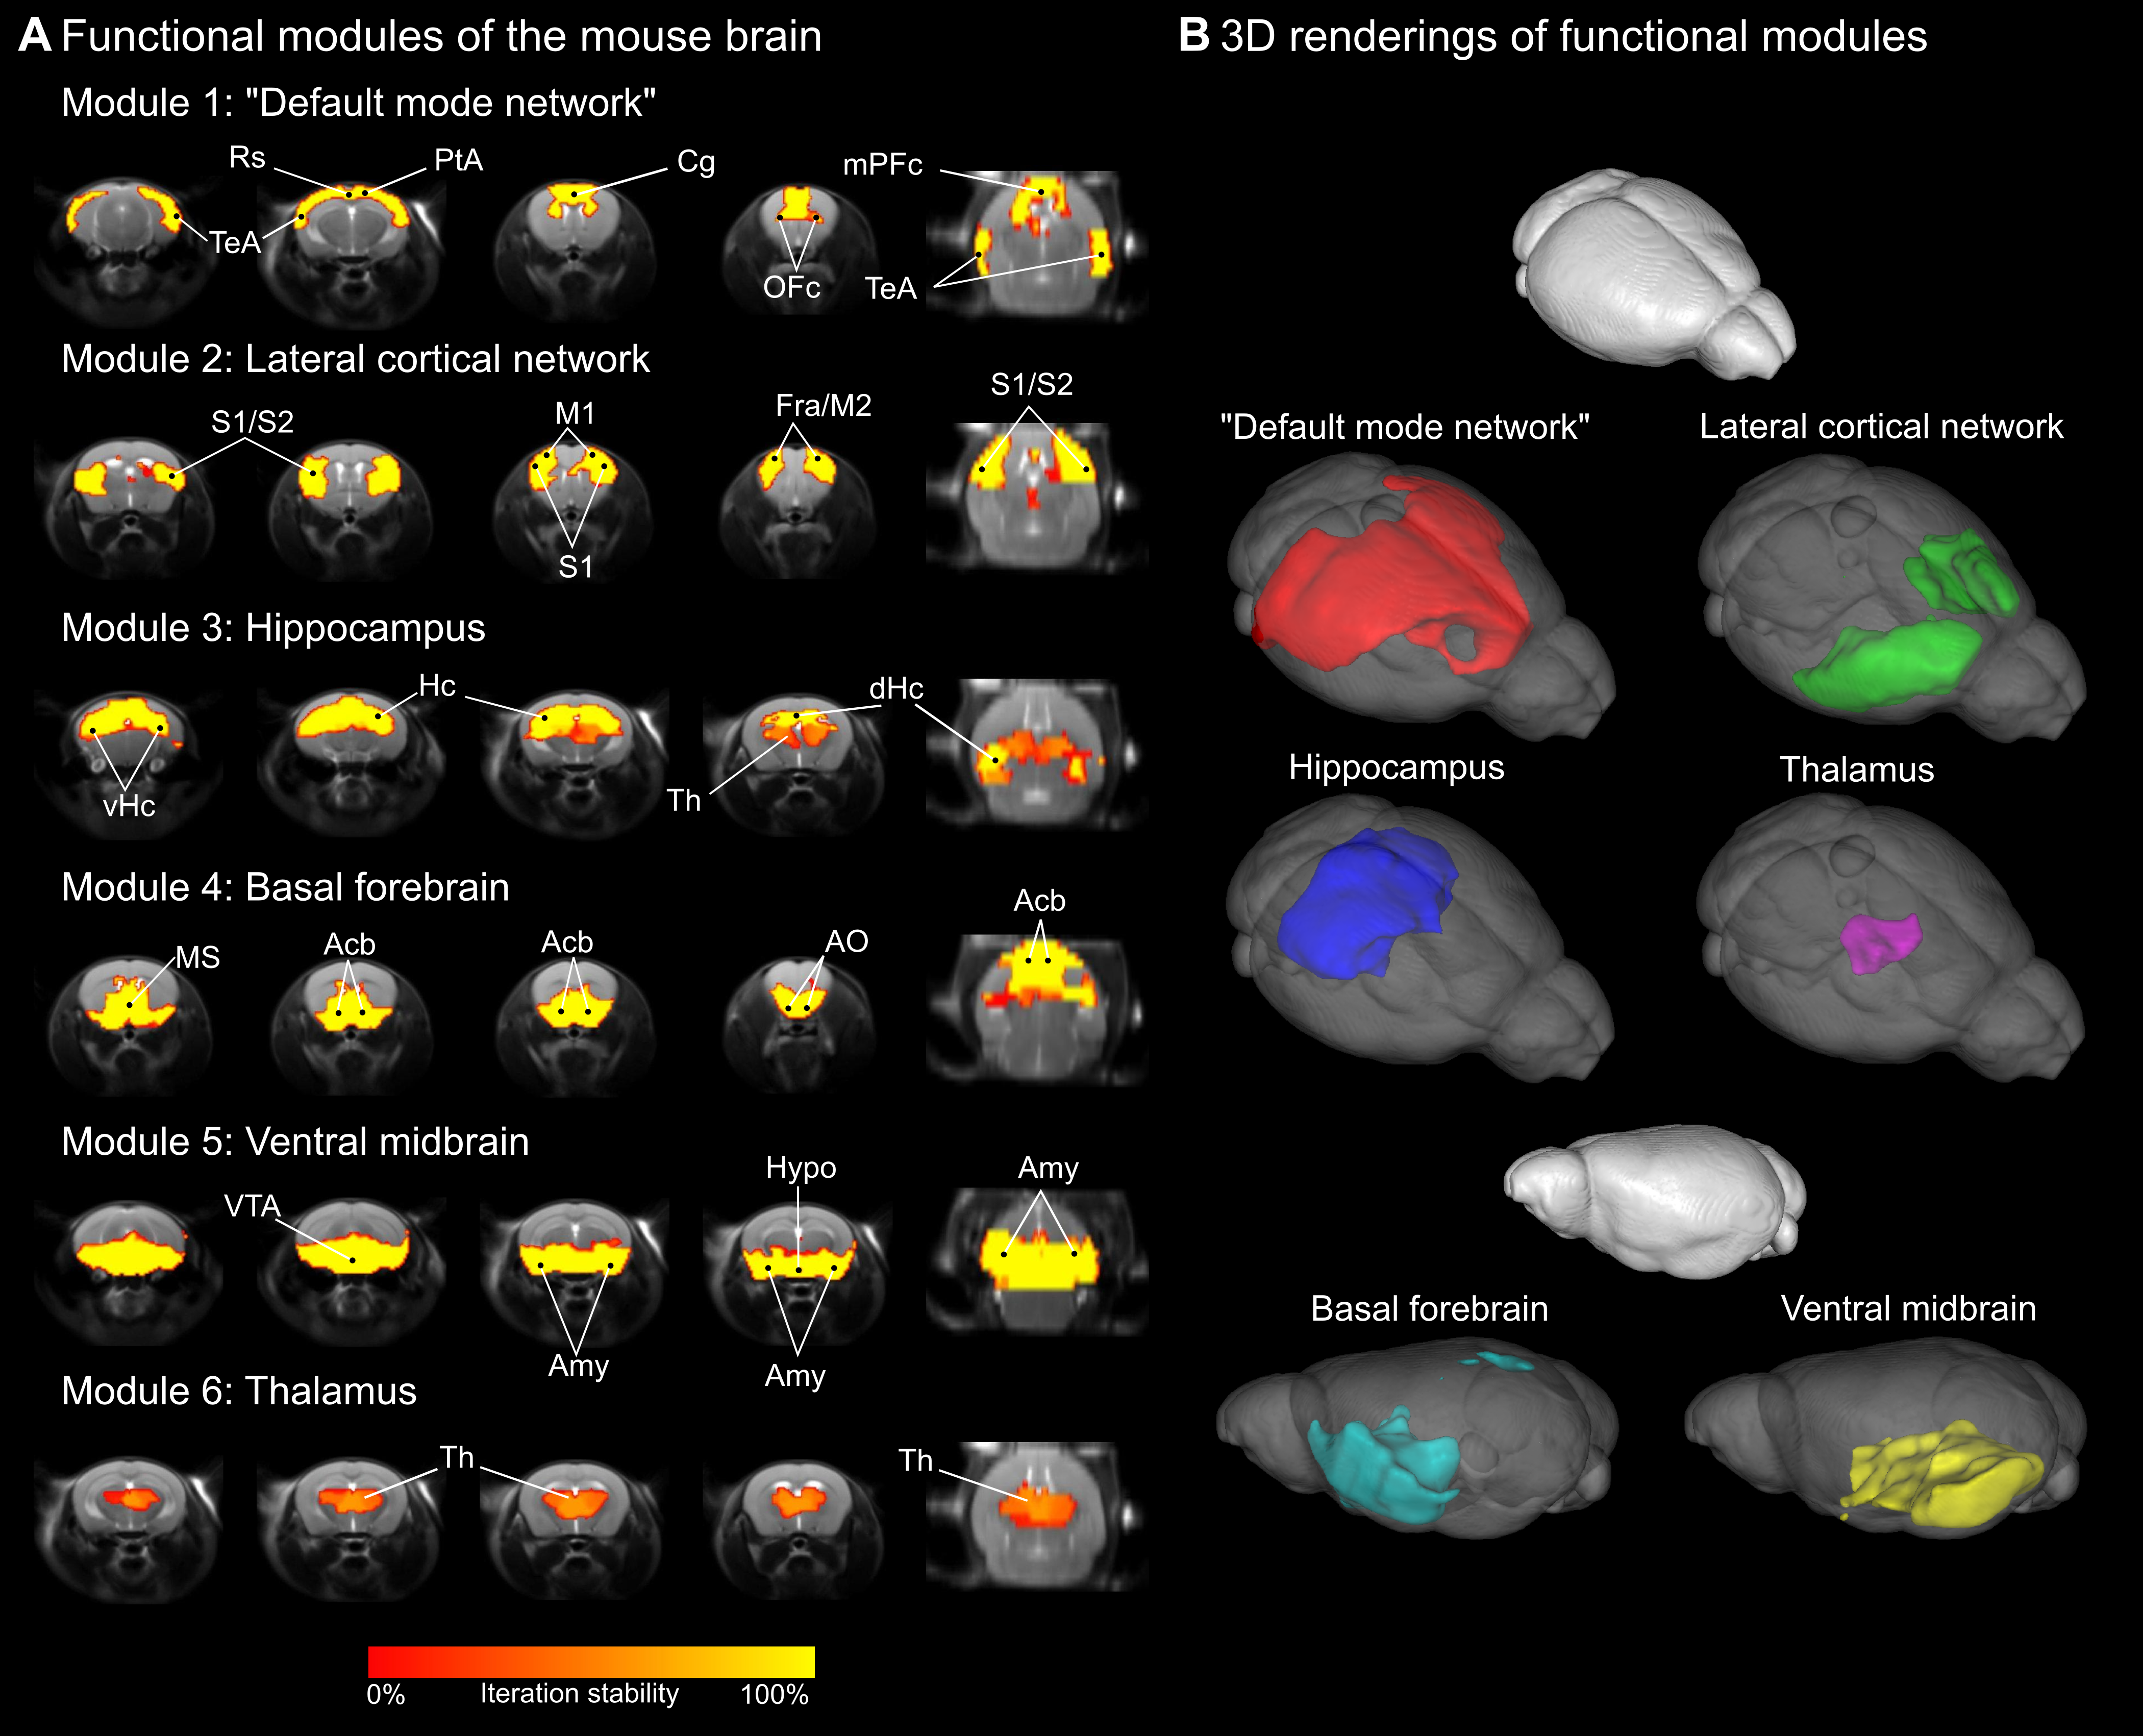
\includegraphics[scale=0.8]{figures/hubs_figure_01_modules_NEW.png}
    \decoRule
    \caption[Functional modules of the mouse brain.]{Functional modules of the
    mouse brain. (\textbf{A}) Module stability maps (100 iterations, N=41
    subjects) overlaid on the anatomical template. For each module, four
    representative coronal slices (left) and one image in the horizontal plane
    (right) are shown. (\textbf{B}) Three-dimensional renderings of the
    reference partition within a transparent brain template. Opaque renderings
    show brain orientation.}
    \label{fig:hubs_fig01_modules}
\end{figure}

\begin{figure}[th]
    \centering
    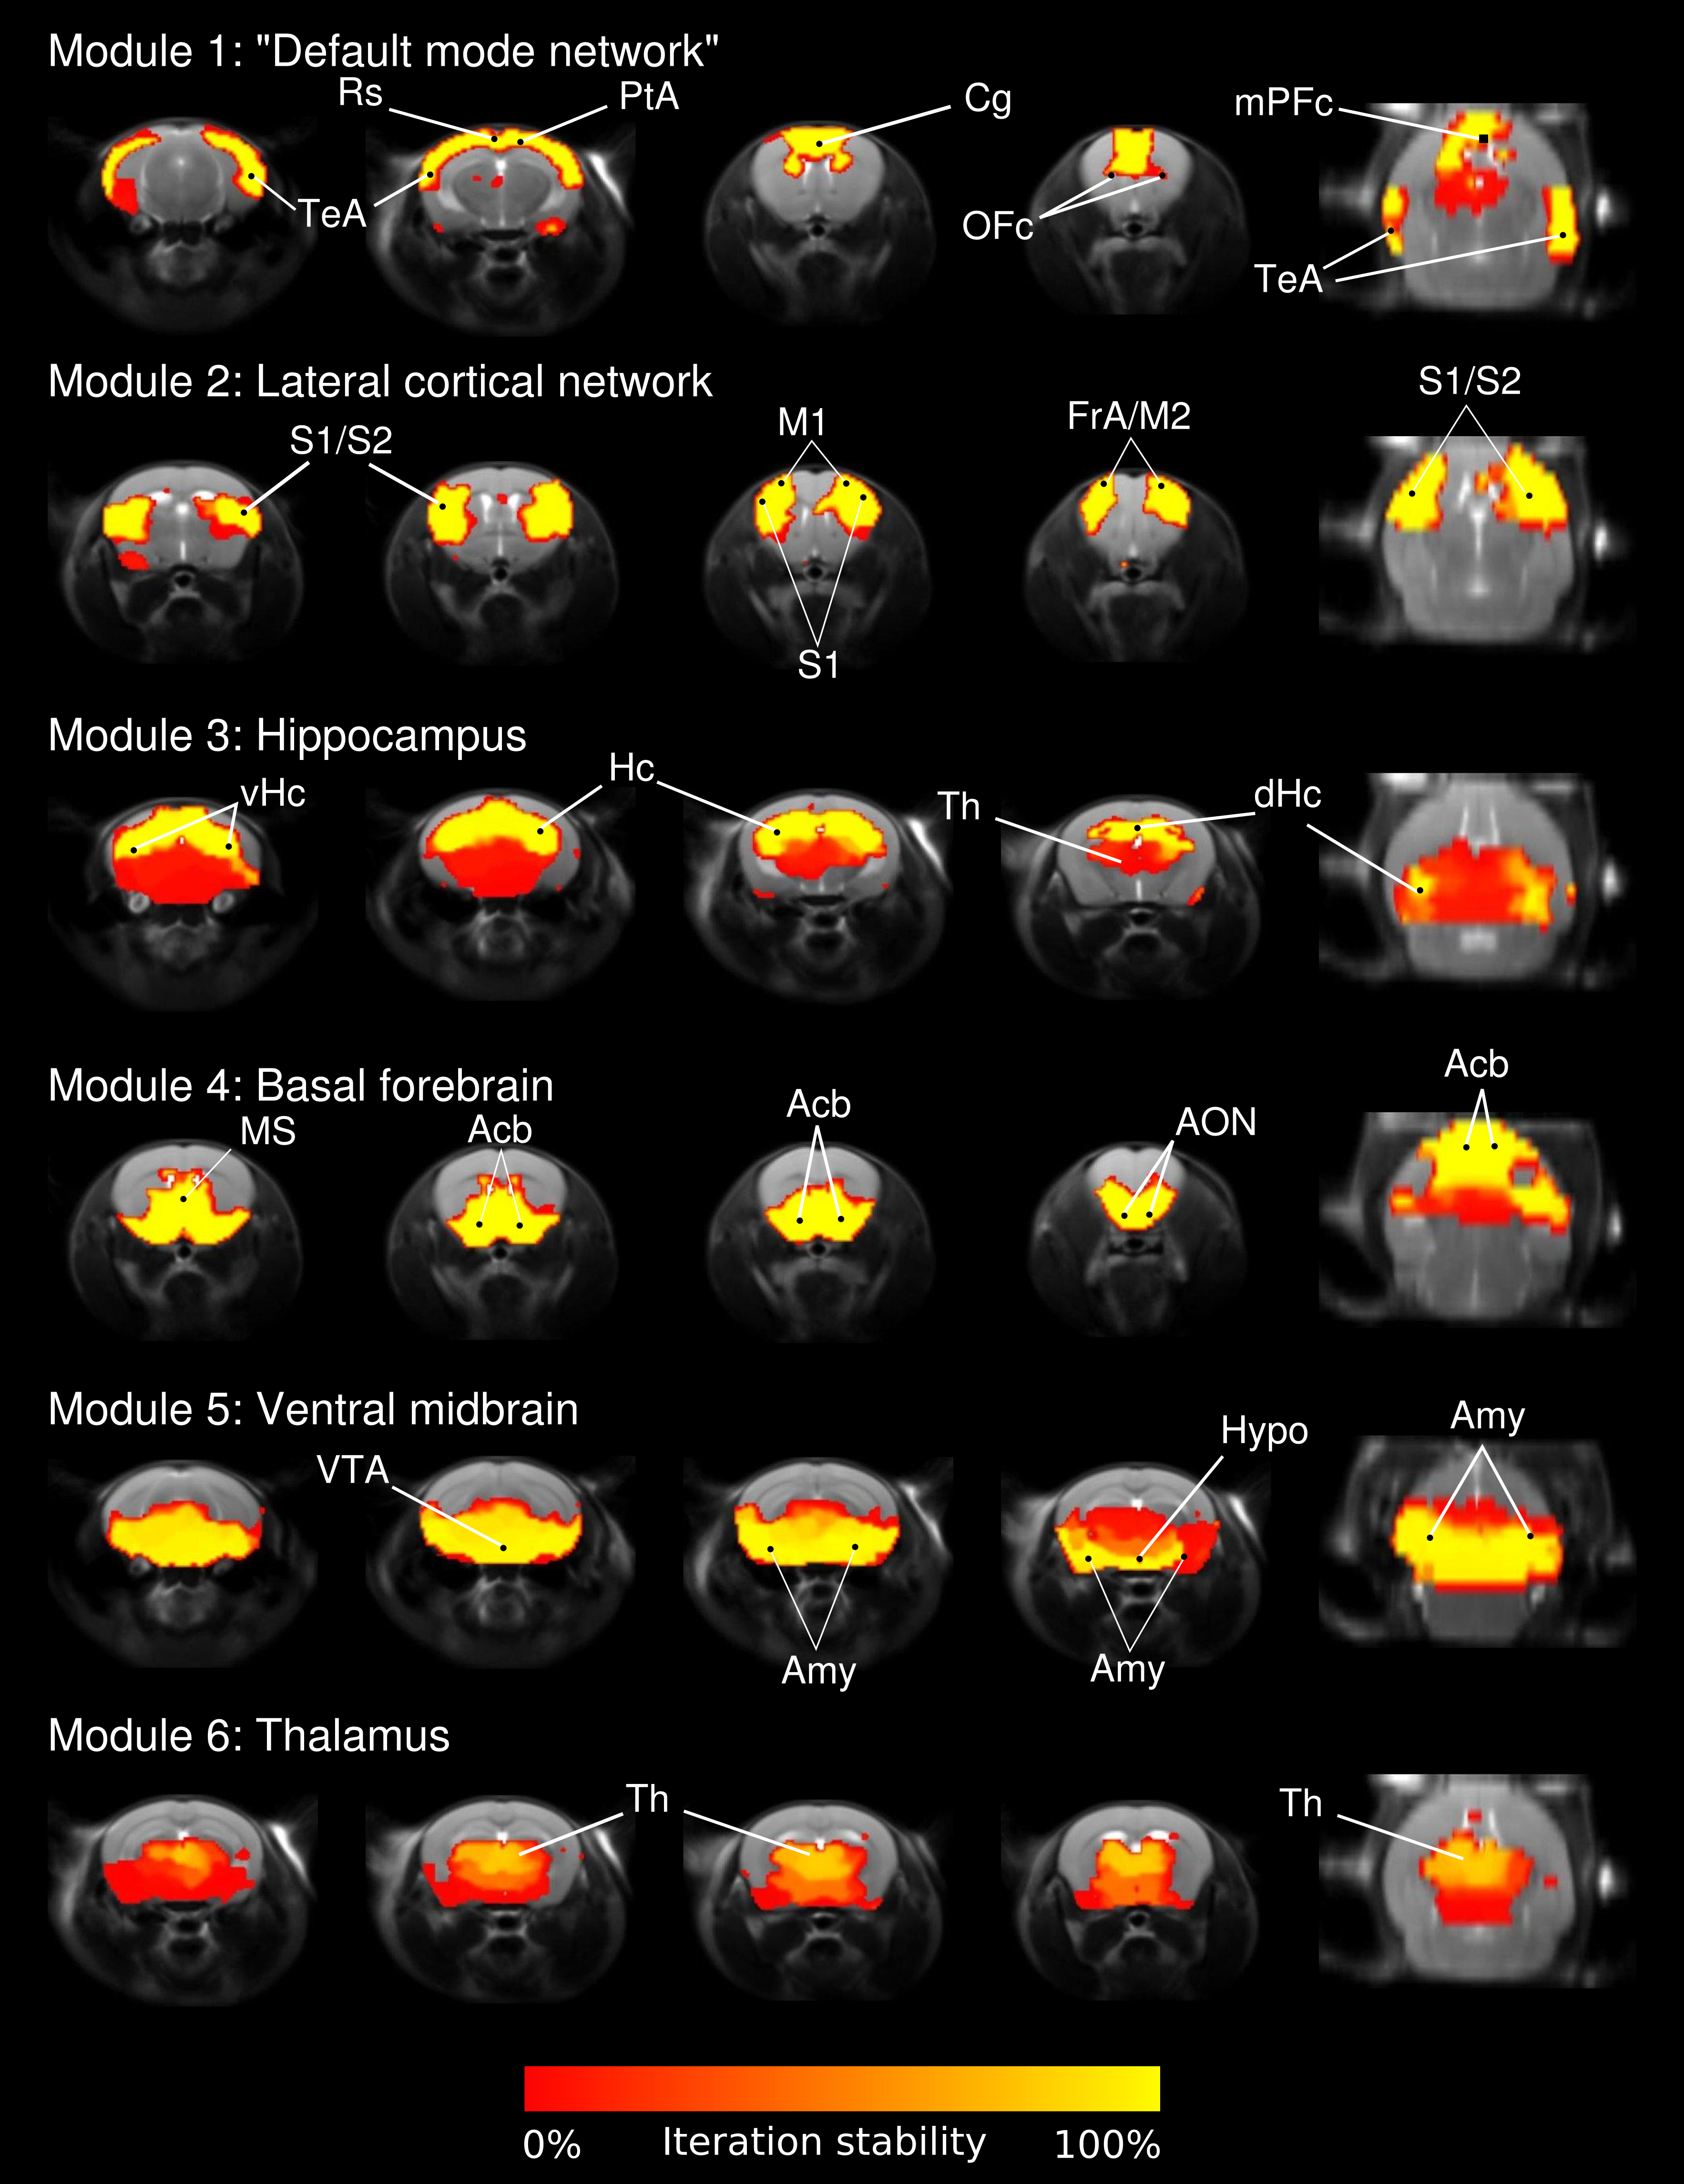
\includegraphics[scale=0.7]{figures/hubs_figure_s2_GSR_modules.png}
    \decoRule
    \caption[Functional modules of the mouse brain computed after global signal
    regression.]{Functional modules of the mouse brain computed after global
    signal regression. Module stability maps (100 iterations, N=41 subjects)
    overlaid on the anatomical template. For each module, four representative
    coronal slices (left) and one image in the horizontal plane (right) are
    shown.}
    \label{fig:hubs_figs2_gsr_modules}
\end{figure}

\begin{figure}[th]
    \centering
    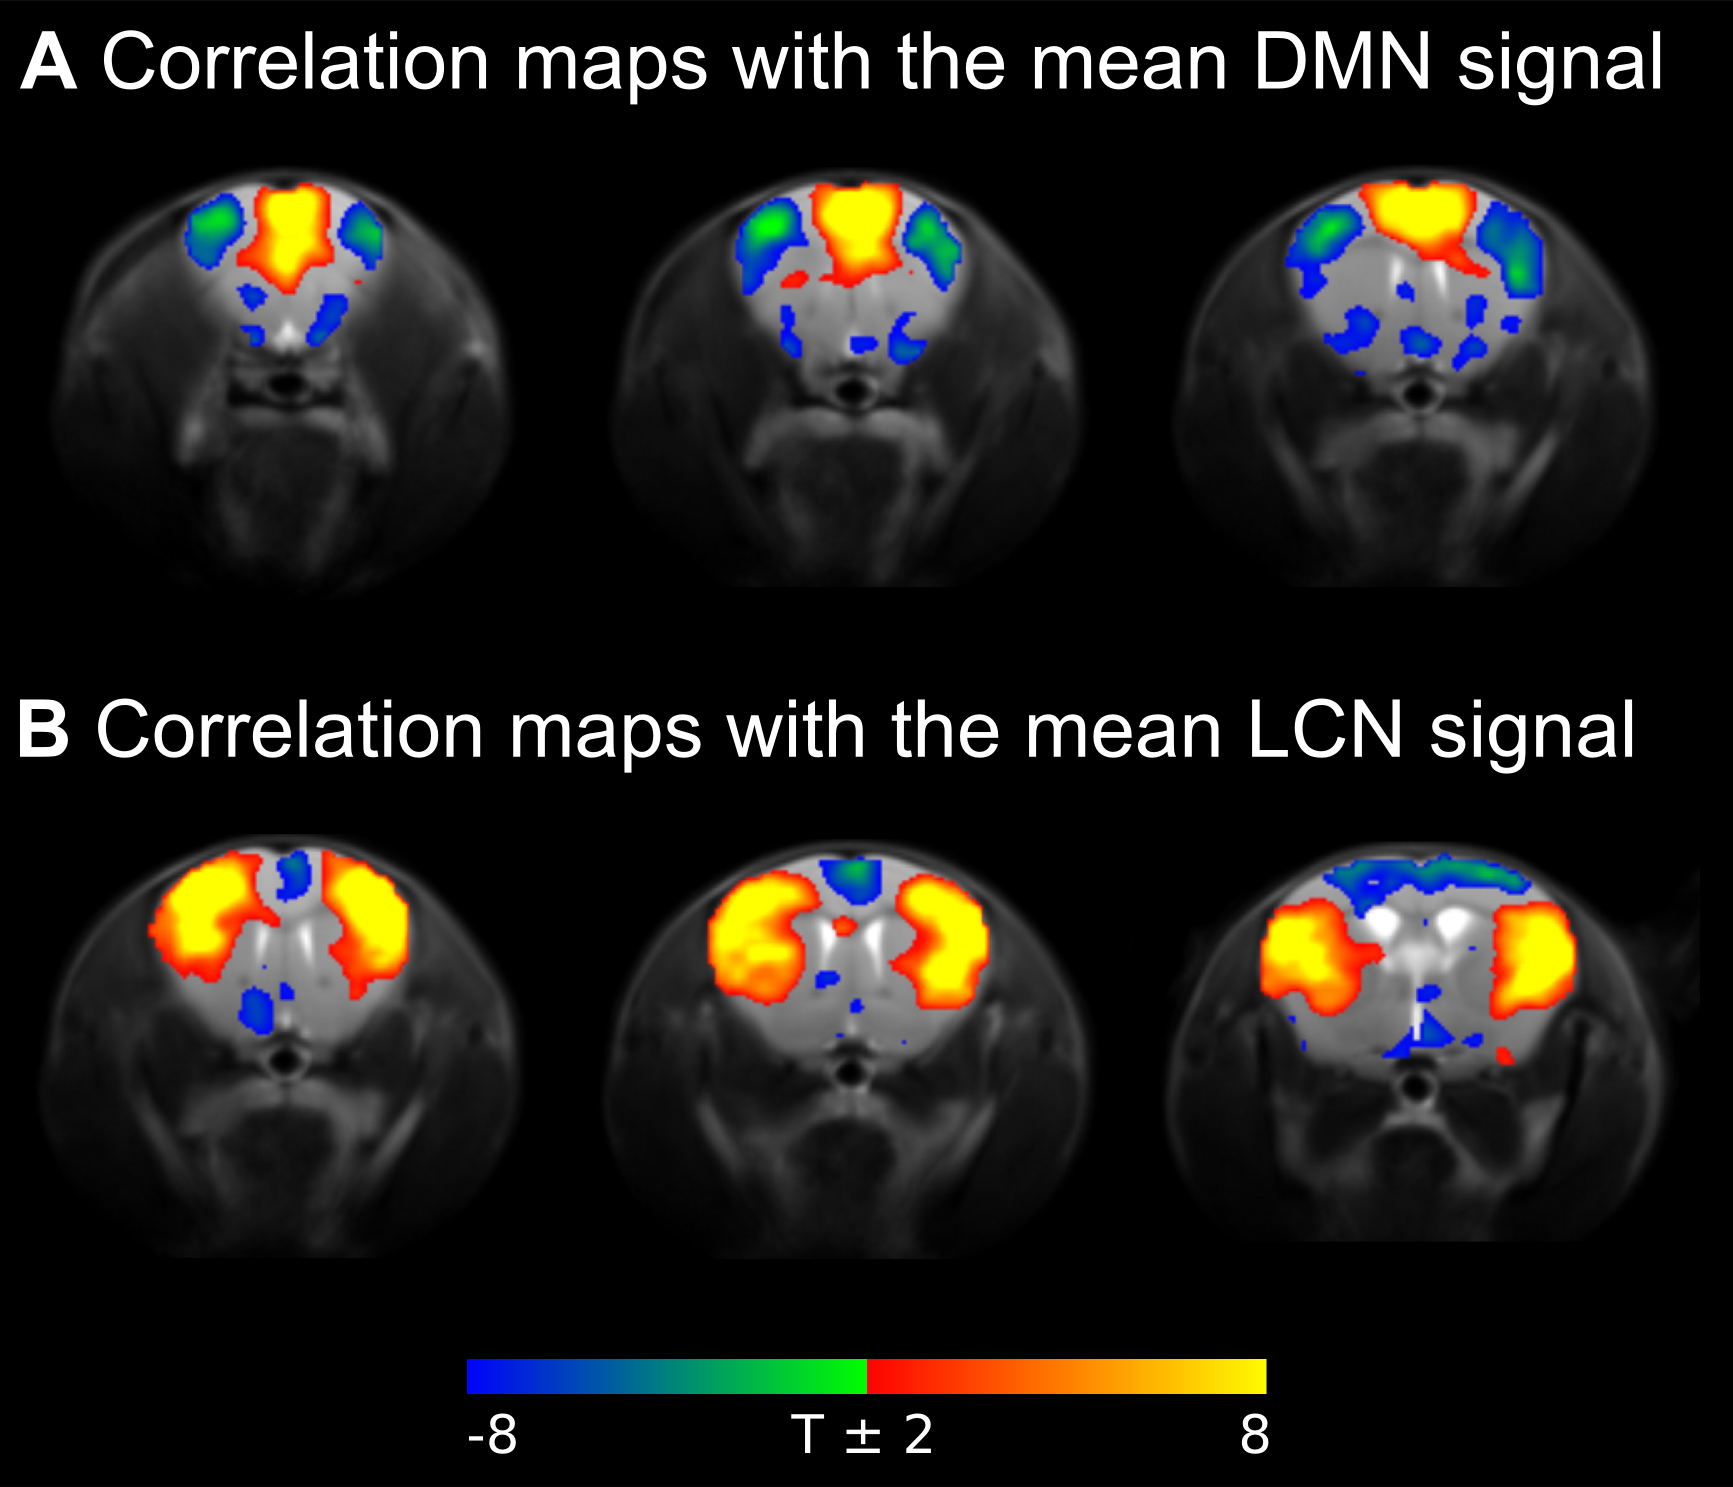
\includegraphics[scale=1]{figures/hubs_figure_s3_dmn_lcn_anticorr.png}
    \decoRule
    \caption[Anticorrelation between the time courses of the default mode and
    lateral cortical networks.]{The two cortical modules identified in the
    study, the default mode network (DMN) and lateral cortical network (LCN),
    are anticorrelated in the dataset with global signal regression.}
    \label{fig:hubs_figs3_anticorrelations}
\end{figure}

To further confirm the robustness of our modular partition, and rule out bias
from spatial smoothing and voxel adjacency artefacts \parencite{power2013} we
carried out a modular partition of functional network in which all connections
shorter than 0.5 mm (approximately 2.5 voxels in plane) were removed, leading to
the identification of a set of modules very consistent with those observed with
full network (Fig.~\ref{fig:hubs_figs4_short_connections}A). With a much more
stringent selection (i.e. removal of connections shorter than 1 mm, ca. 5 voxels
in plane) modular instability was observed for subcortical modules, with
evidence of stable partitioning of the DMN and thalamic modules as a single
joint community (Fig.~\ref{fig:hubs_figs4_short_connections}B). This modular structure is consistent with previous
seed-based rsfMRI studies of the mouse brain, in which thalamic areas appear to
be strongly correlated with cingulate and retrosplenial cingulate cortices
\parencite{sforazzini2016}. The appearance of subcortical modular instability
upon removal of 1 mm connections is not unexpected, because 1 mm long
connections cover the anatomical extension of some of the anatomical structures
that constitute individual functional modules (e.g.  radial hippocampus, or
thalamus) \parencite{paxinos2004}. 

\begin{figure}[th]
    \centering
    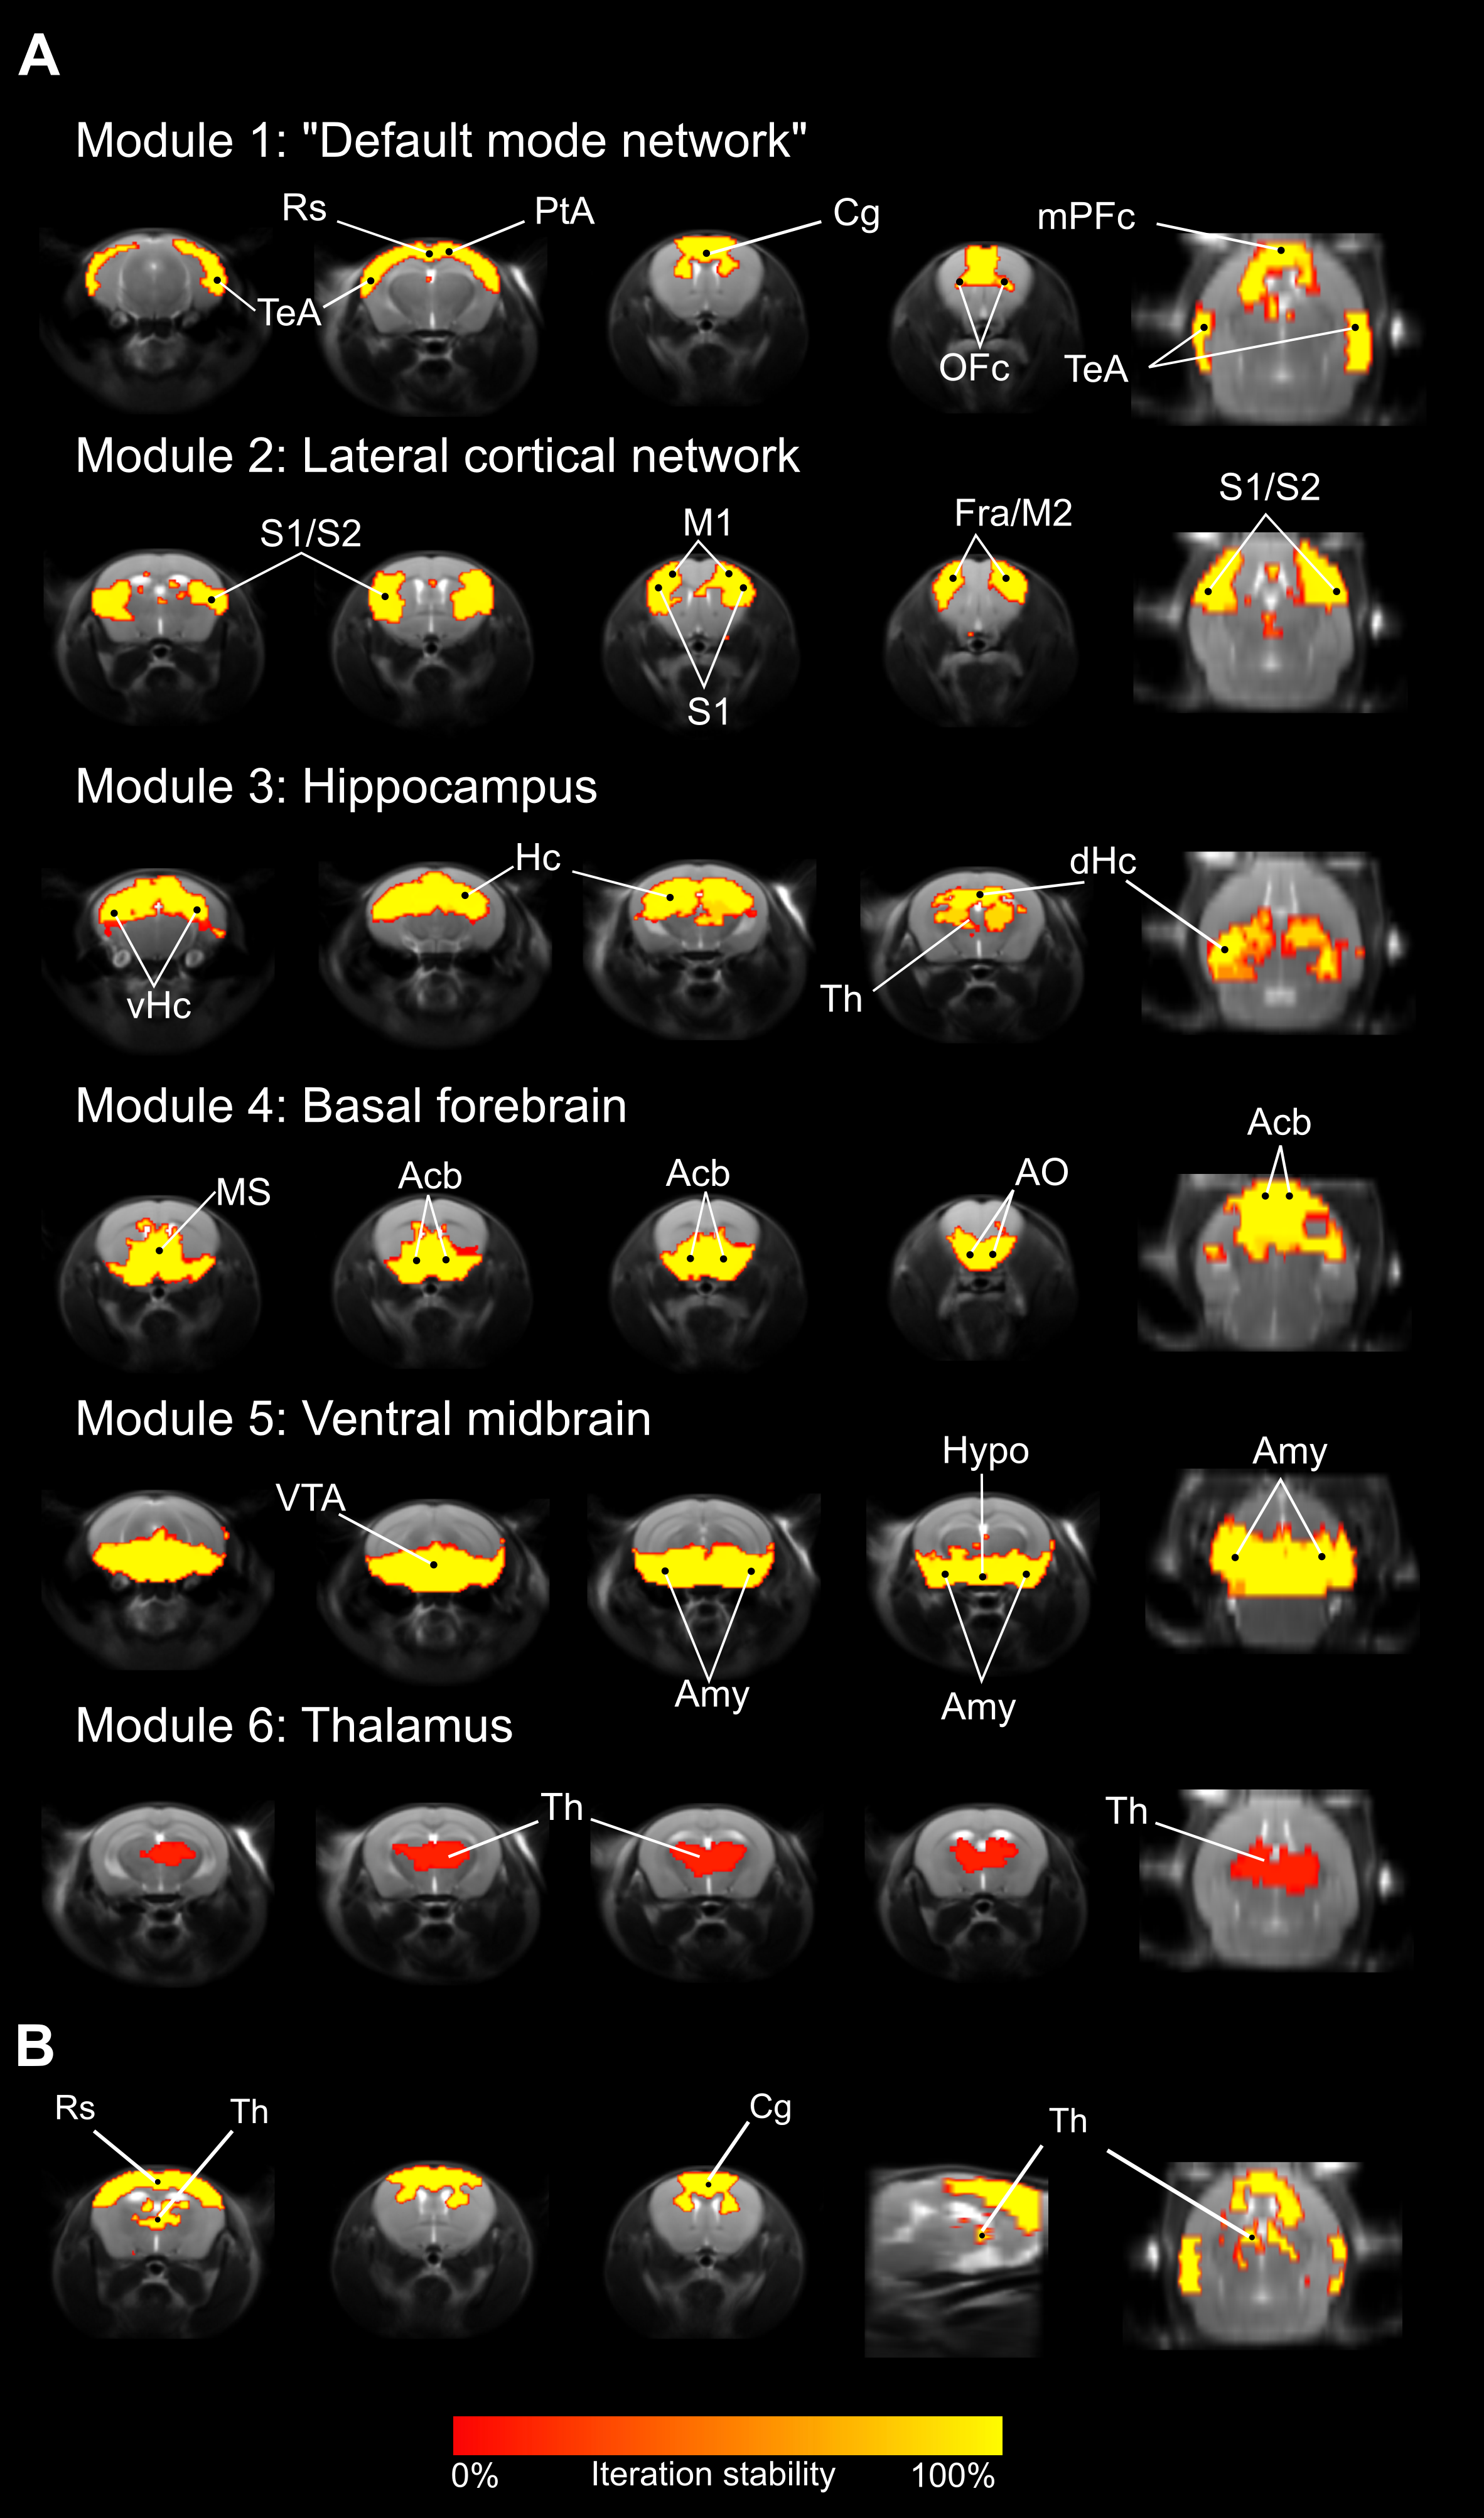
\includegraphics[scale=0.85]{figures/hubs_figure_s4_modules_short_edges_removed.png}
    \decoRule
    \caption[Modules of the mouse brain upon removal of short
    connections.]{Modules of the mouse brain upon removal of short connections.
    (\textbf{A}) Connections shorter than 0.5 mm were removed. (\textbf{B}) DMN
    module in the functional network upon removal of connections shorter than
    1.0 mm. Module stability maps (100 iterations, N=41 subjects) are overlaid
    on the anatomical template.}
    \label{fig:hubs_figs4_short_connections}
\end{figure}


\subsection{Global functional hubs are located in cingulate and prefrontal
cortex}

To identify functional hubs at a voxel scale, we first mapped connection
strength values for all nodes in the functional network \parencite{rubinov2011}.
In agreement with human studies \parencite{tomasi2011}, cortical and subcortical
regions appeared to have distinct connectional profiles, with the former
exhibiting much higher strength overall (Fig.~\ref{fig:hubs_fig2_global_hubs}A).
Anatomical maps of the voxels exhibiting the highest strength ($p < 0.0001$, FDR
corrected) revealed foci of high connection strength in several sub-regions of
the DMN network, including prefrontal, anterior and posterior cingulate cortex
as well as parietal association regions (Fig.~\ref{fig:hubs_fig2_global_hubs}B). 

\begin{figure}[th]
    \centering
    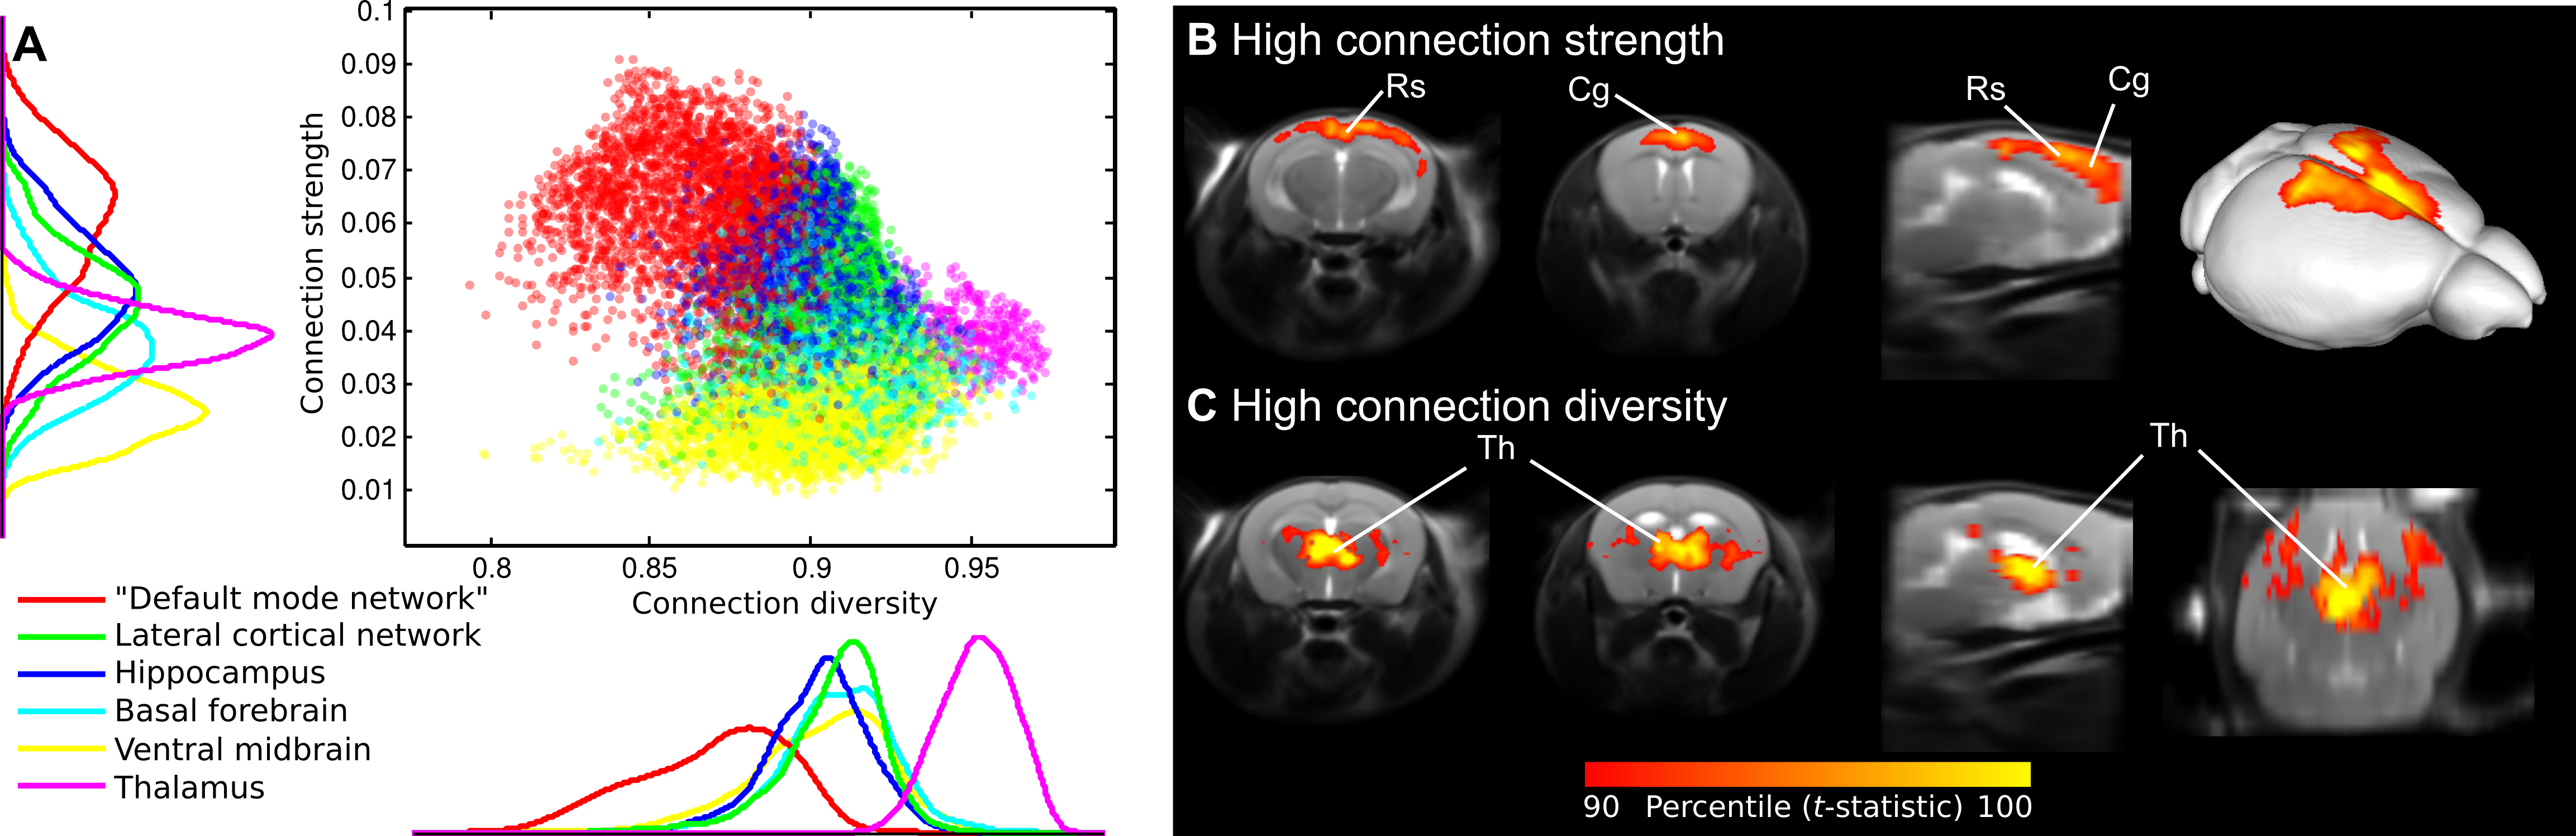
\includegraphics[scale=0.7]{figures/hubs_figure_02_hubs_global_NEW.png}
    \decoRule
    \caption[Global hubs of the mouse brain.]{Global hubs of the mouse brain.
    (\textbf{A}) Connection diversity and connection strength values are plotted
    for all nodes in the average functional network. Nodes are colour-coded
    according to their module. (\textbf{B}) Nodes surviving the top percentage
    threshold for connection strength are shown on two images in the coronal
    view (left), one image in the sagittal view (middle), and on a
    three-dimensional cortical surface rendering. (\textbf{C}) Nodes surviving
    the top percentage threshold for connection diversity are shown on two
    images in the coronal view, one image in the sagittal view (left), one image
    in the sagittal view (middle), and on a three-dimensional cortical surface
    rendering.}
    \label{fig:hubs_fig2_global_hubs}
\end{figure}


To account for potential bias induced by coil-induced regional variation in
temporal signal to noise ratio (tSNR), we performed connection strength mapping
on rsfMRI timeseries corrupted with random pink noise such to achieve homogenous
tSNR levels equalling values observed in deep subcortical areas ($\approx 25$).
The results of this analysis confirmed the original hub locations ($p < 0.0038$,
FDR corrected, Fig.~\ref{fig:hubs_figs5_snr}) thus ruling out a significant
contribution of coil-related bias on high strength connection maps.

\begin{figure}[th]
    \centering
    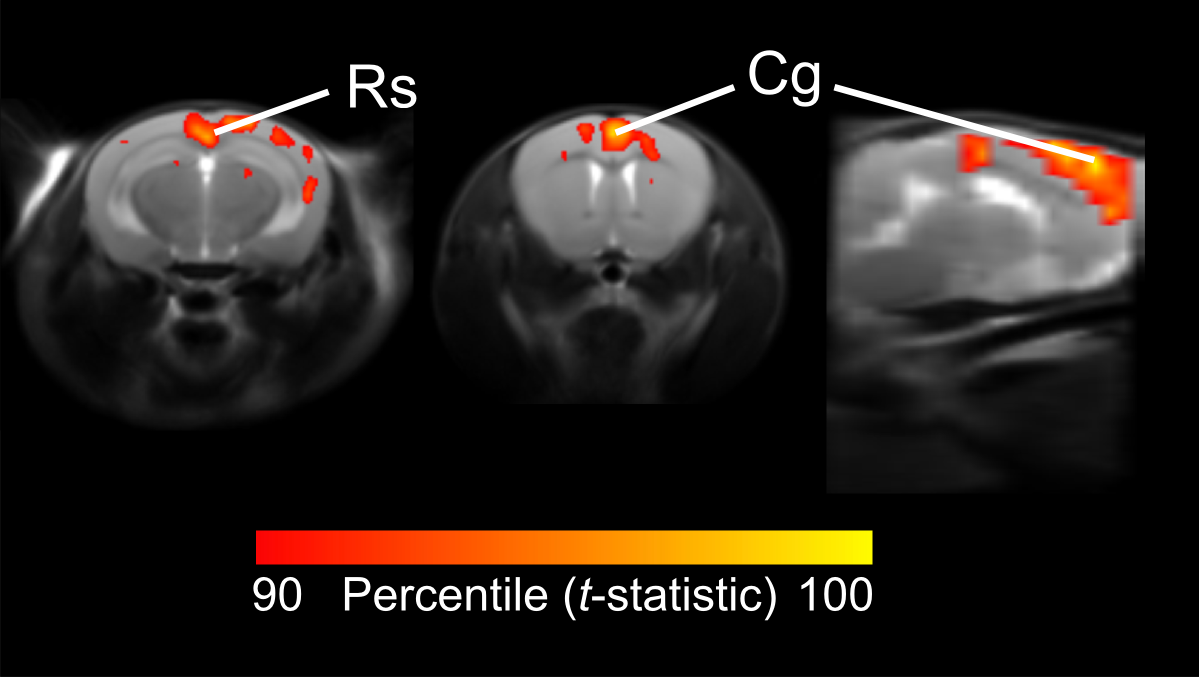
\includegraphics[scale=1.2]{figures/hubs_figure_s5_snr.png}
    \decoRule
    \caption[High-strength nodes in rsfMRI time series after tSNR corruption
    with pink noise.]{High-strength nodes in rsfMRI time series after tSNR
    corruption with pink noise. The final timeseries had tSNR values similar to
    those observed in deep brain areas furthest to the surface coil array
    ($\approx 25$).  In spite of this, cingulate and retrosplenial areas emerged
    as regions with highest global connectivity strength.}
    \label{fig:hubs_figs5_snr}
\end{figure}

\subsection{High connection diversity hubs are located in the thalamus and
associative cortical areas}

Connection diversity is a network attribute used to identify nodes participating
in multiple functional sub-networks \parencite{power2013, rubinov2011}.
Whole-brain mapping of nodes exhibiting high connection diversity ($p < 0.001$,
FDR corrected) revealed a prominent involvement of thalamic areas
(Fig.~\ref{fig:hubs_fig2_global_hubs}A,C), a finding consistent with the
integrative and relay functions subserved by this region
\parencite{draganski2008}. 

To extrapolate and compare our results with human studies, where topological
analyses are typically limited to cortical regions, we also generated a map of
high connection diversity voxels within the identified neocortical modules
(Fig.~\ref{fig:hubs_fig3_cortical_hubs}). As recently described in humans
\parencite{power2011}, nodes within the DMN module exhibited low average
connection diversity, suggesting an extensive internal integration of this
module and its function as a highly efficient “processing” system. Importantly,
the approach also led to the identification of spatially restricted foci of high
connection diversity the temporal association cortex ($p < 0.001$, FDR corrected),
a cortical area serving prominent integrative roles. Consistent with recent
human studies \parencite{power2013}, foci of high connection diversity were also
found in the anterior insular cortex ($p < 0.032$, uncorrected), although in this
region the effect appeared to be less robust and did not survive FDR correction
($p < 0.2905$, FDR corrected).

\begin{figure}[th]
    \centering
    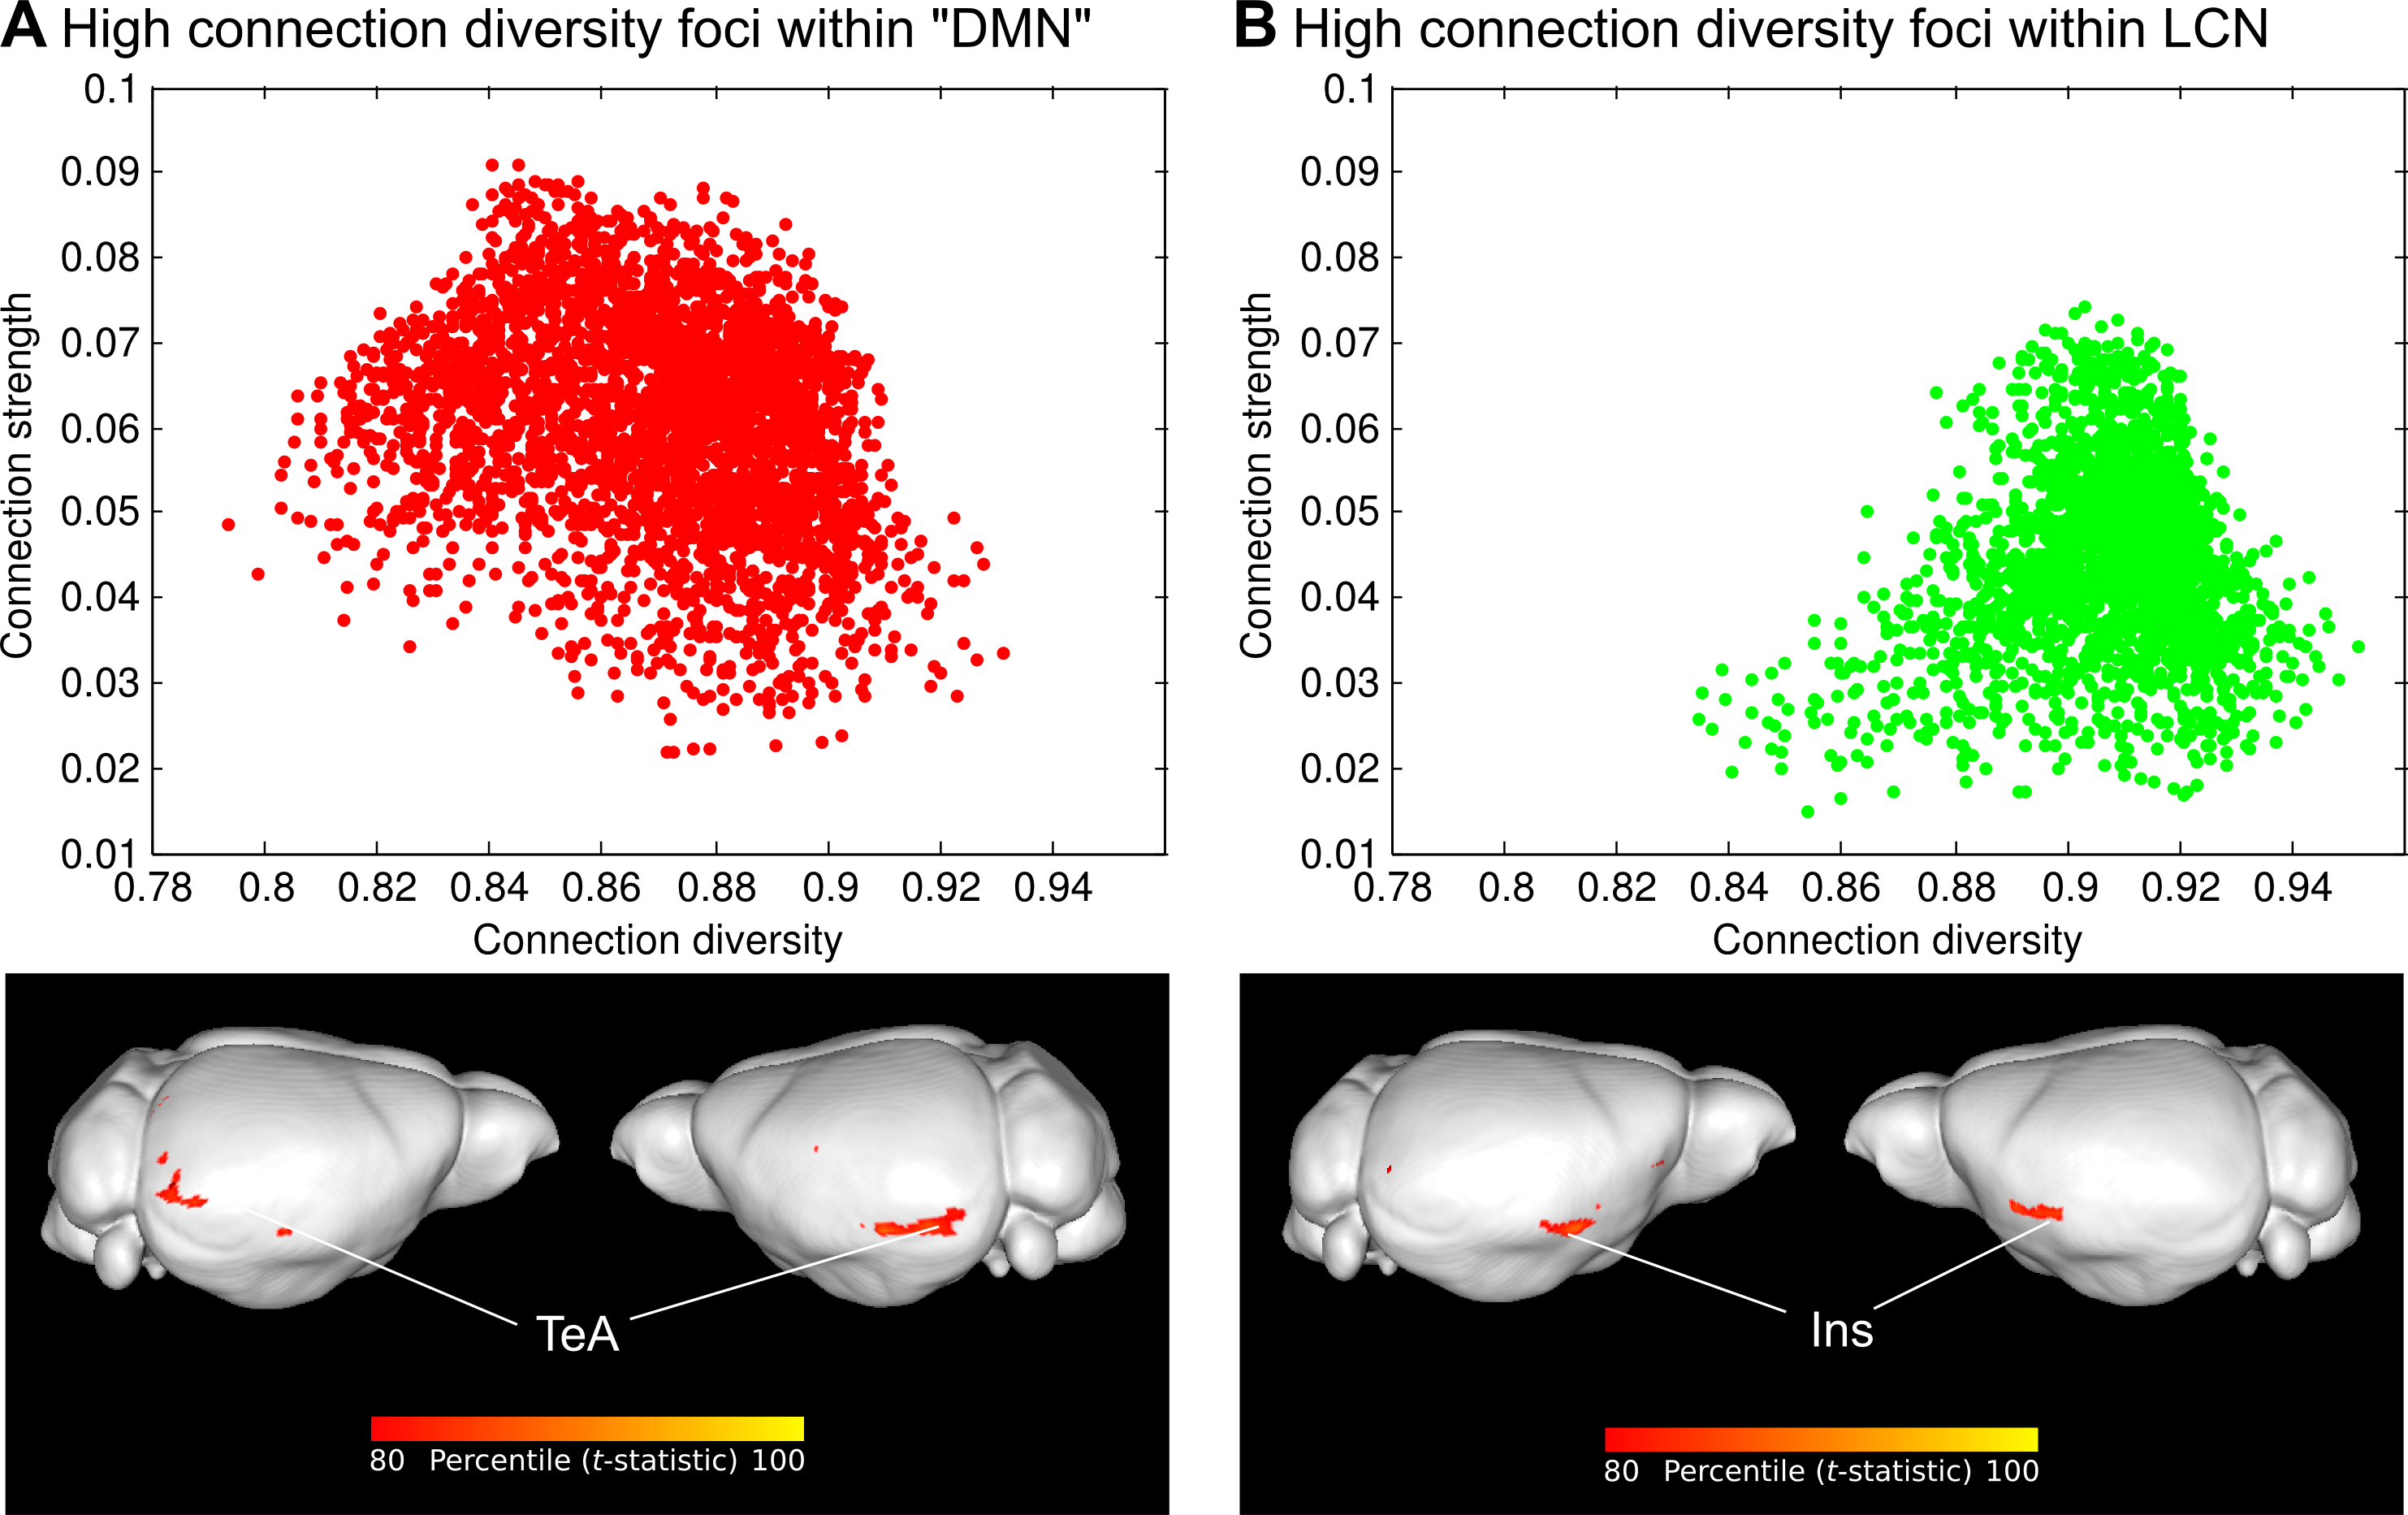
\includegraphics[scale=1.1]{figures/hubs_figure_03_cortical_hubs_NEW.png}
    \decoRule
    \caption[High connection diversity regions within cortical modules.]{High
    connection diversity regions within cortical modules. Connection diversity
    and strength values (calculated in the average functional network) are
    plotted for all nodes in the “default mode network” (\textbf{A}) and the
    lateral cortical network (\textbf{B}). Bottom panels highlight brain nodes
    surviving the top percentage threshold within each of the two cortical. The
    nodes are shown as three dimensional renderings on the cortical surface.}
    \label{fig:hubs_fig3_cortical_hubs}
\end{figure}

\subsection{Intra-module mapping of high connection hubs}

To further investigate the topological organization of the individual
sub-networks, we mapped, for each of the identified modules, voxels
characterised by high within-module connectivity strength, which we refer to as
“module hubs” (Fig.~\ref{fig:hubs_fig4_module_hubs}). The top 10 \% voxels were
statistically highly significant for all the modules, with the exception of the
ventral midbrain module, where the FDR corrected p-value was, however, very
close to significance level (DMN: $p < 0.000011$, LCN: $p < 0.00039$, Hc: $p <
0.0016$, basal forebrain: $p < 0.0068$, ventral midbrain: $p < 0.0572$, thalamus: $p <
0.0000096$, all FDR corrected). Module hub mapping in the DMN and lateral
cortical networks highlighted high within-module strength foci in the anterior
cingulate cortex, and frontal association cortices, respectively. Additional
candidate module hubs were identified in the dorsal hippocampus (hippocampal
module), nucleus accumbens and olfactory nuclei (basal ganglia), pons/ventral
subiculum (ventral midbrain), and centromedial thalamic nuclei (thalamus). 

\begin{figure}[th]
    \centering
    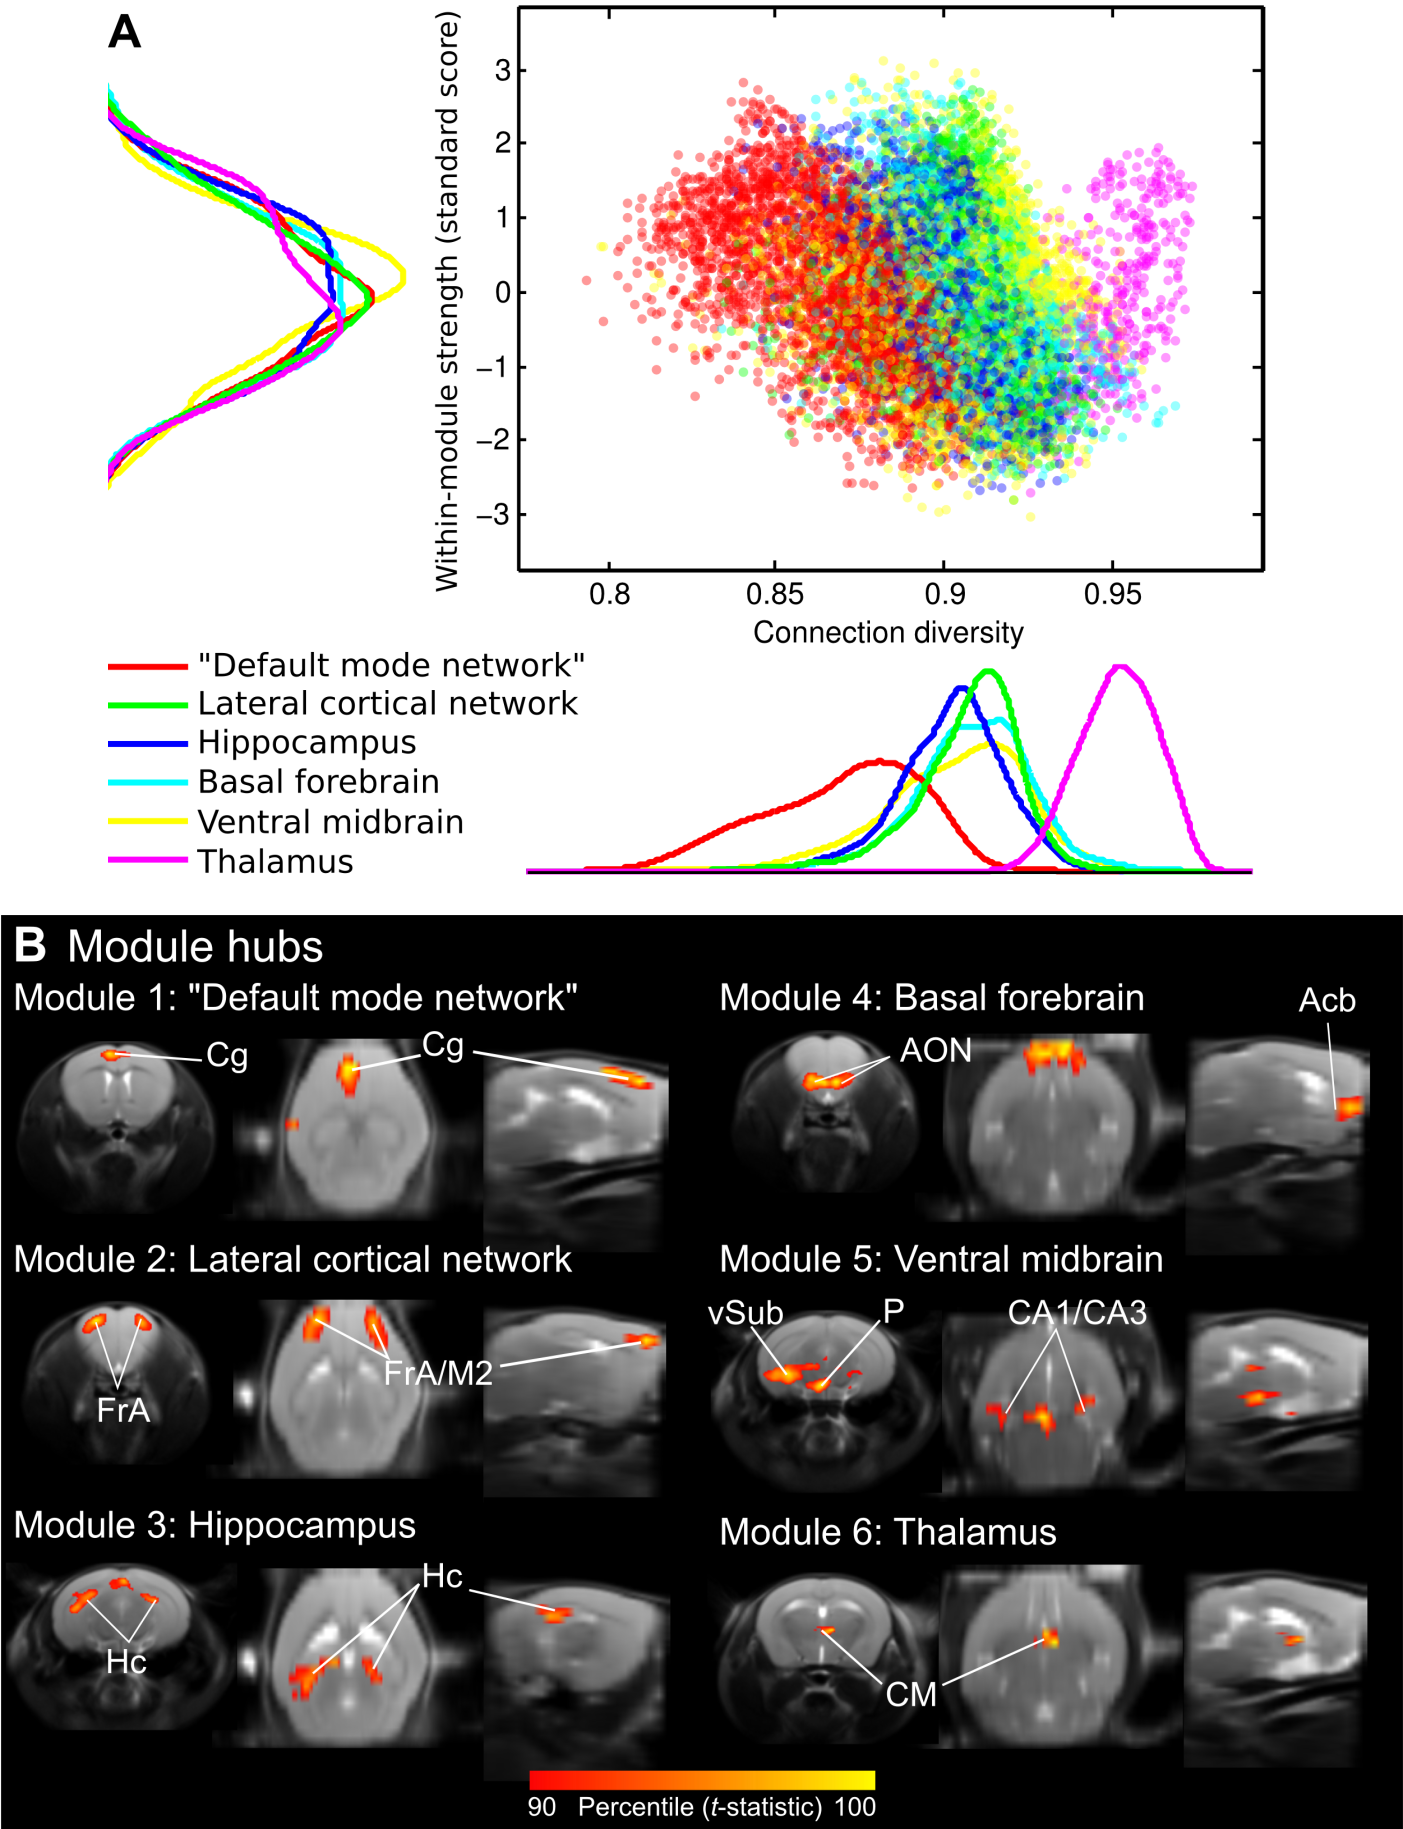
\includegraphics[scale=0.6]{figures/hubs_figure_04_module_hubs_NEW.png}
    \decoRule
    \caption[Module hubs.]{Module hubs. (\textbf{A}) Connection diversity and
    normalised (z) scores of within-module strength plotted for all nodes in the
    average functional network. Nodes are colour-coded according to their
    module.  (\textbf{B}) For each module, nodes surviving the top percentage
    threshold are shown on images in representative axial, horizontal and
    sagittal views of the mouse brain.}
    \label{fig:hubs_fig4_module_hubs}
\end{figure}

\subsection{Reproducibility of global and intra-module hub mapping on smaller
subject cohorts}

In order to evaluate the reproducibility of global and intra-module hub mapping
on smaller subject cohorts, 100 random subject subsets each with exactly N=10
animals were generated, and global and intra-module hub regions were mapped
independently for each group. The results show robust conservation of most hub
locations across the vast majority of randomly-generated 10-subject groups for
global and module hubs (Fig.~\ref{fig:hubs_figs6_reproducibility}). Diversity
hubs within the two cortical modules exhibited lower conservation, reflecting
intrinsic lower stability and significance levels these integrative locations as
reported above. 

\begin{figure}[th]
    \centering
    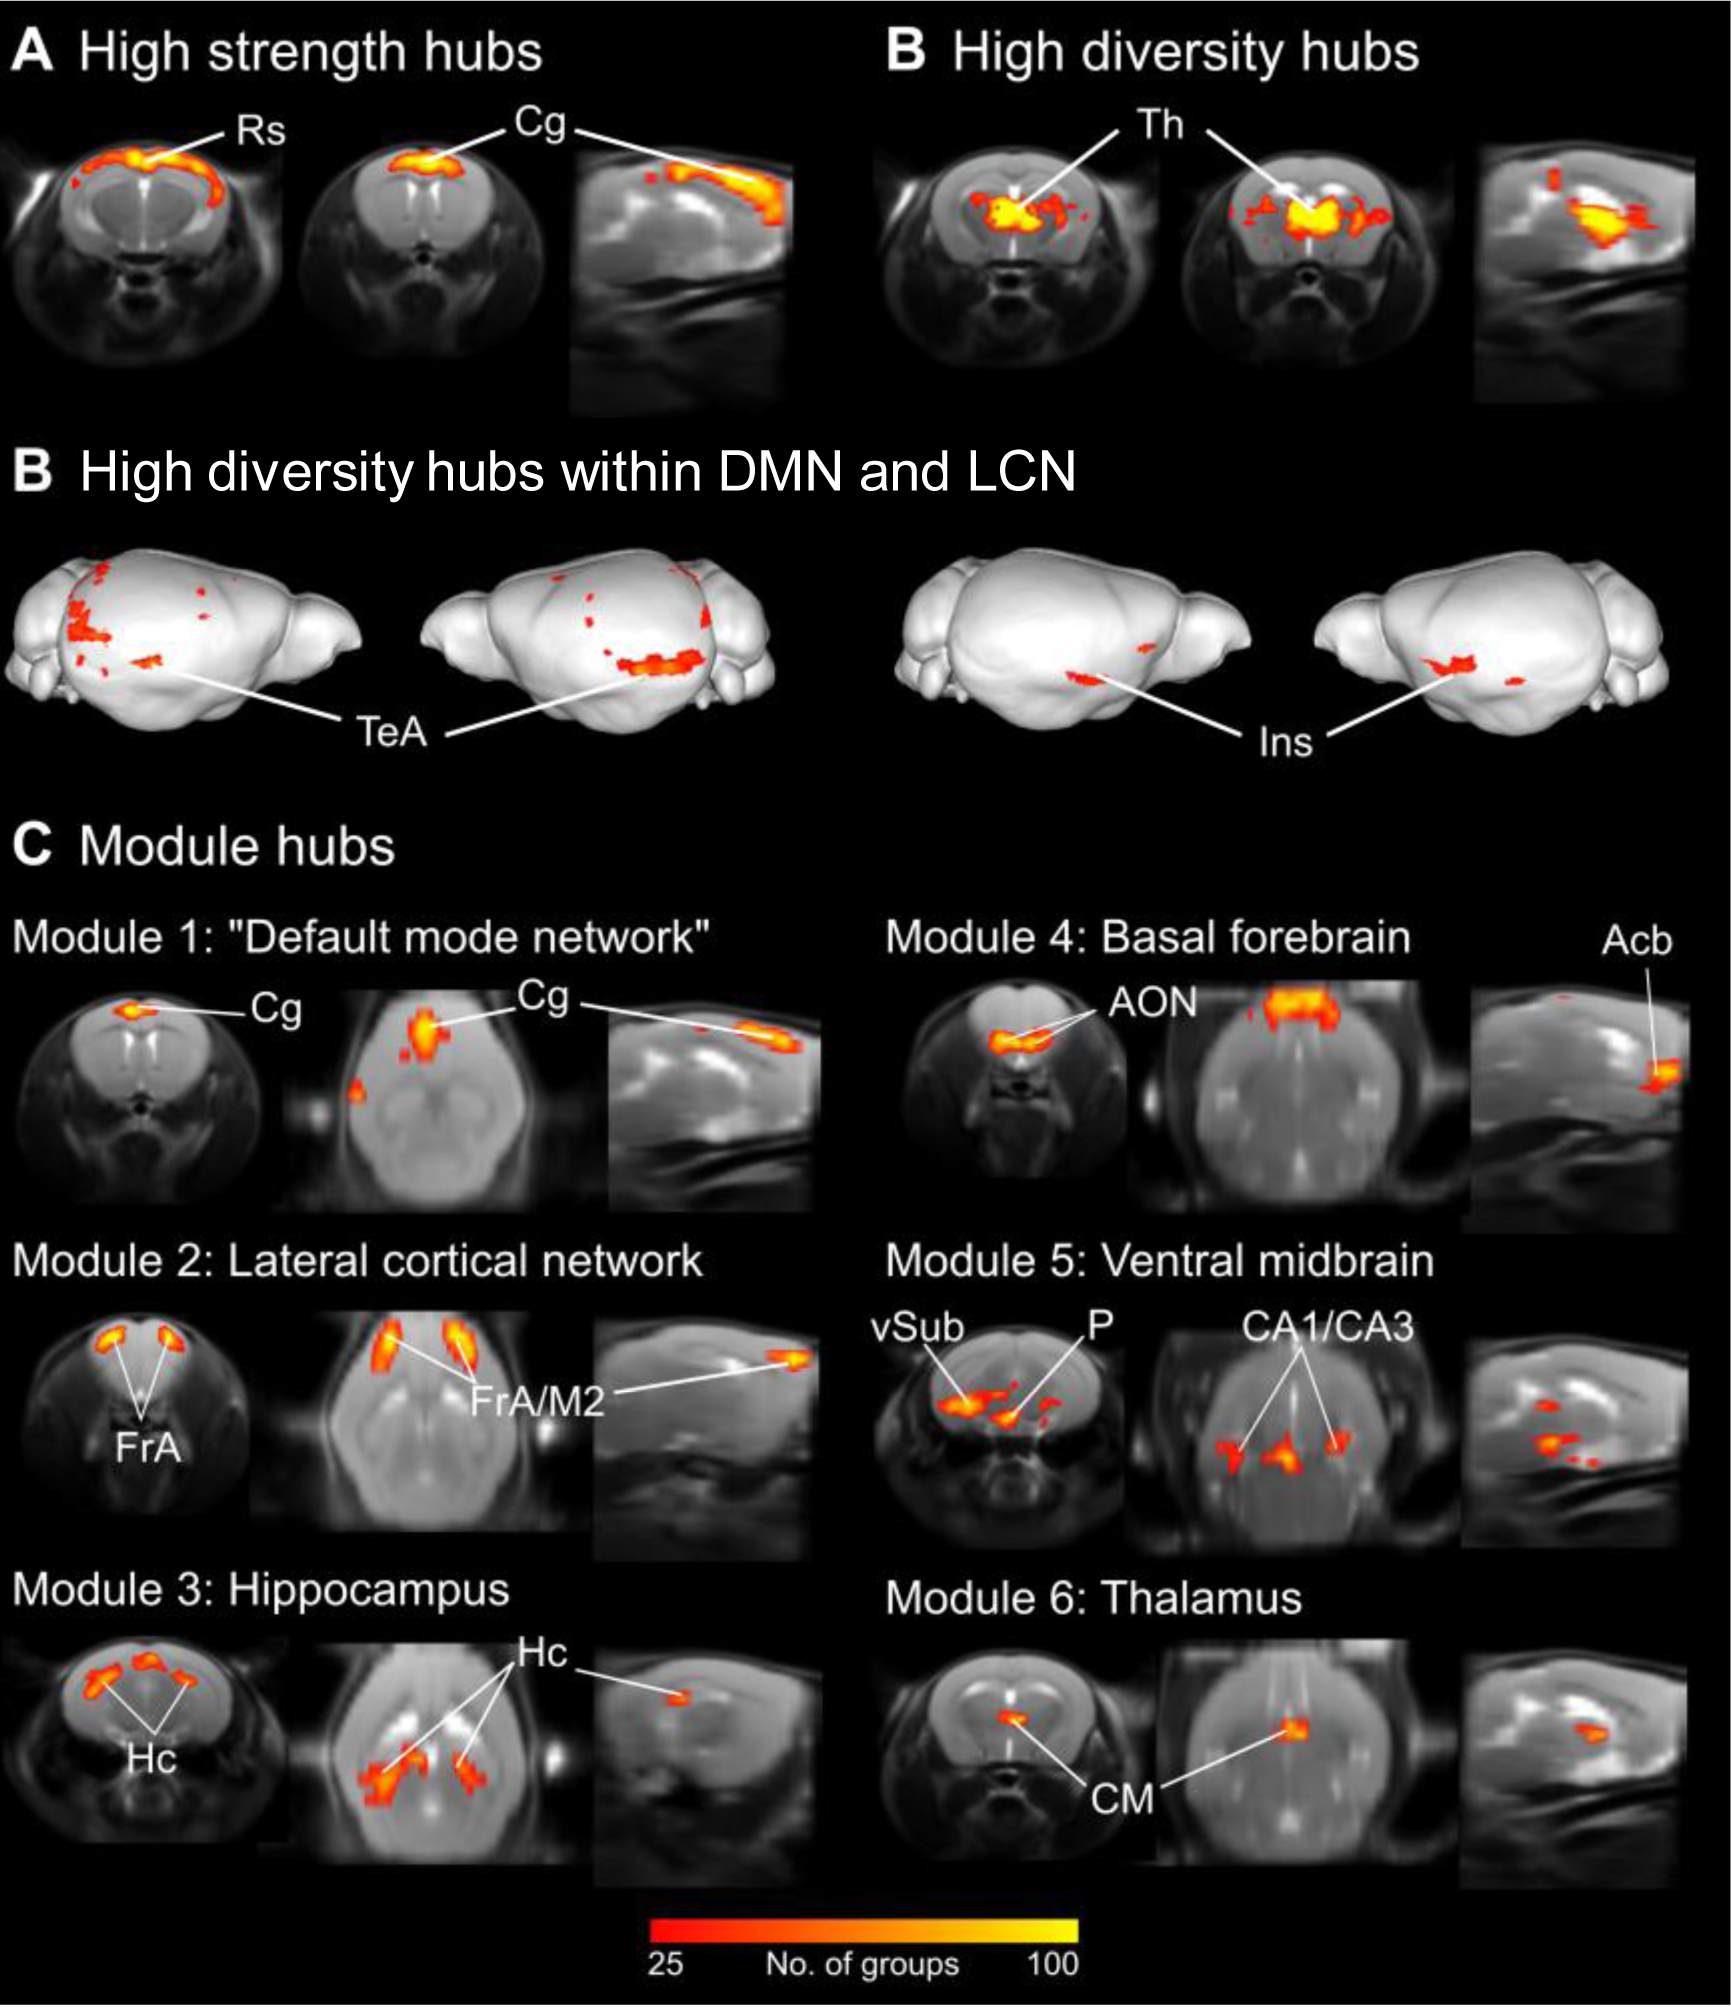
\includegraphics[scale=0.8]{figures/hubs_figure_s6_hub_reproducibility_10_animals_NEW.png}
    \decoRule
    \caption[Reproducibility of functional hubs in random sub-groups of 10
    animals.]{Reproducibility of functional hubs in random sub-groups of 10
    animals. The voxel maps express the number of groups (out of 100 random
    10-animal partitions of the original 41-subject cohort) in which a given
    voxel was identified as belonging to a hub of the given type.}
    \label{fig:hubs_figs6_reproducibility}
\end{figure}

\subsection{The identified hubs are mutually and preferentially interconnected}

To assess the presence of mutual inter-module connections between the identified
hubs, the anatomical correspondence between the strongest connections of each
source hub seed (Fig.~\ref{fig:hubs_figs1_seed_location}) and the independently
determined hub foci in other modules was investigated
(Fig.~\ref{fig:hubs_fig5_hub_connectivity}). For the majority of the candidate
hub pairs, the strongest connections of the source hub overlapped with voxels
identified above as foci of maximal within module strength or connection
diversity. This finding of robust and preferential hub-hub connections suggests
that these brain regions act as a tightly interconnected sub-network within the
mouse brain (Fig.~\ref{fig:hubs_fig6_hub_relationshiops}A,C), underpinning cross-module integrative functions.

\begin{figure}[th]
    \centering
    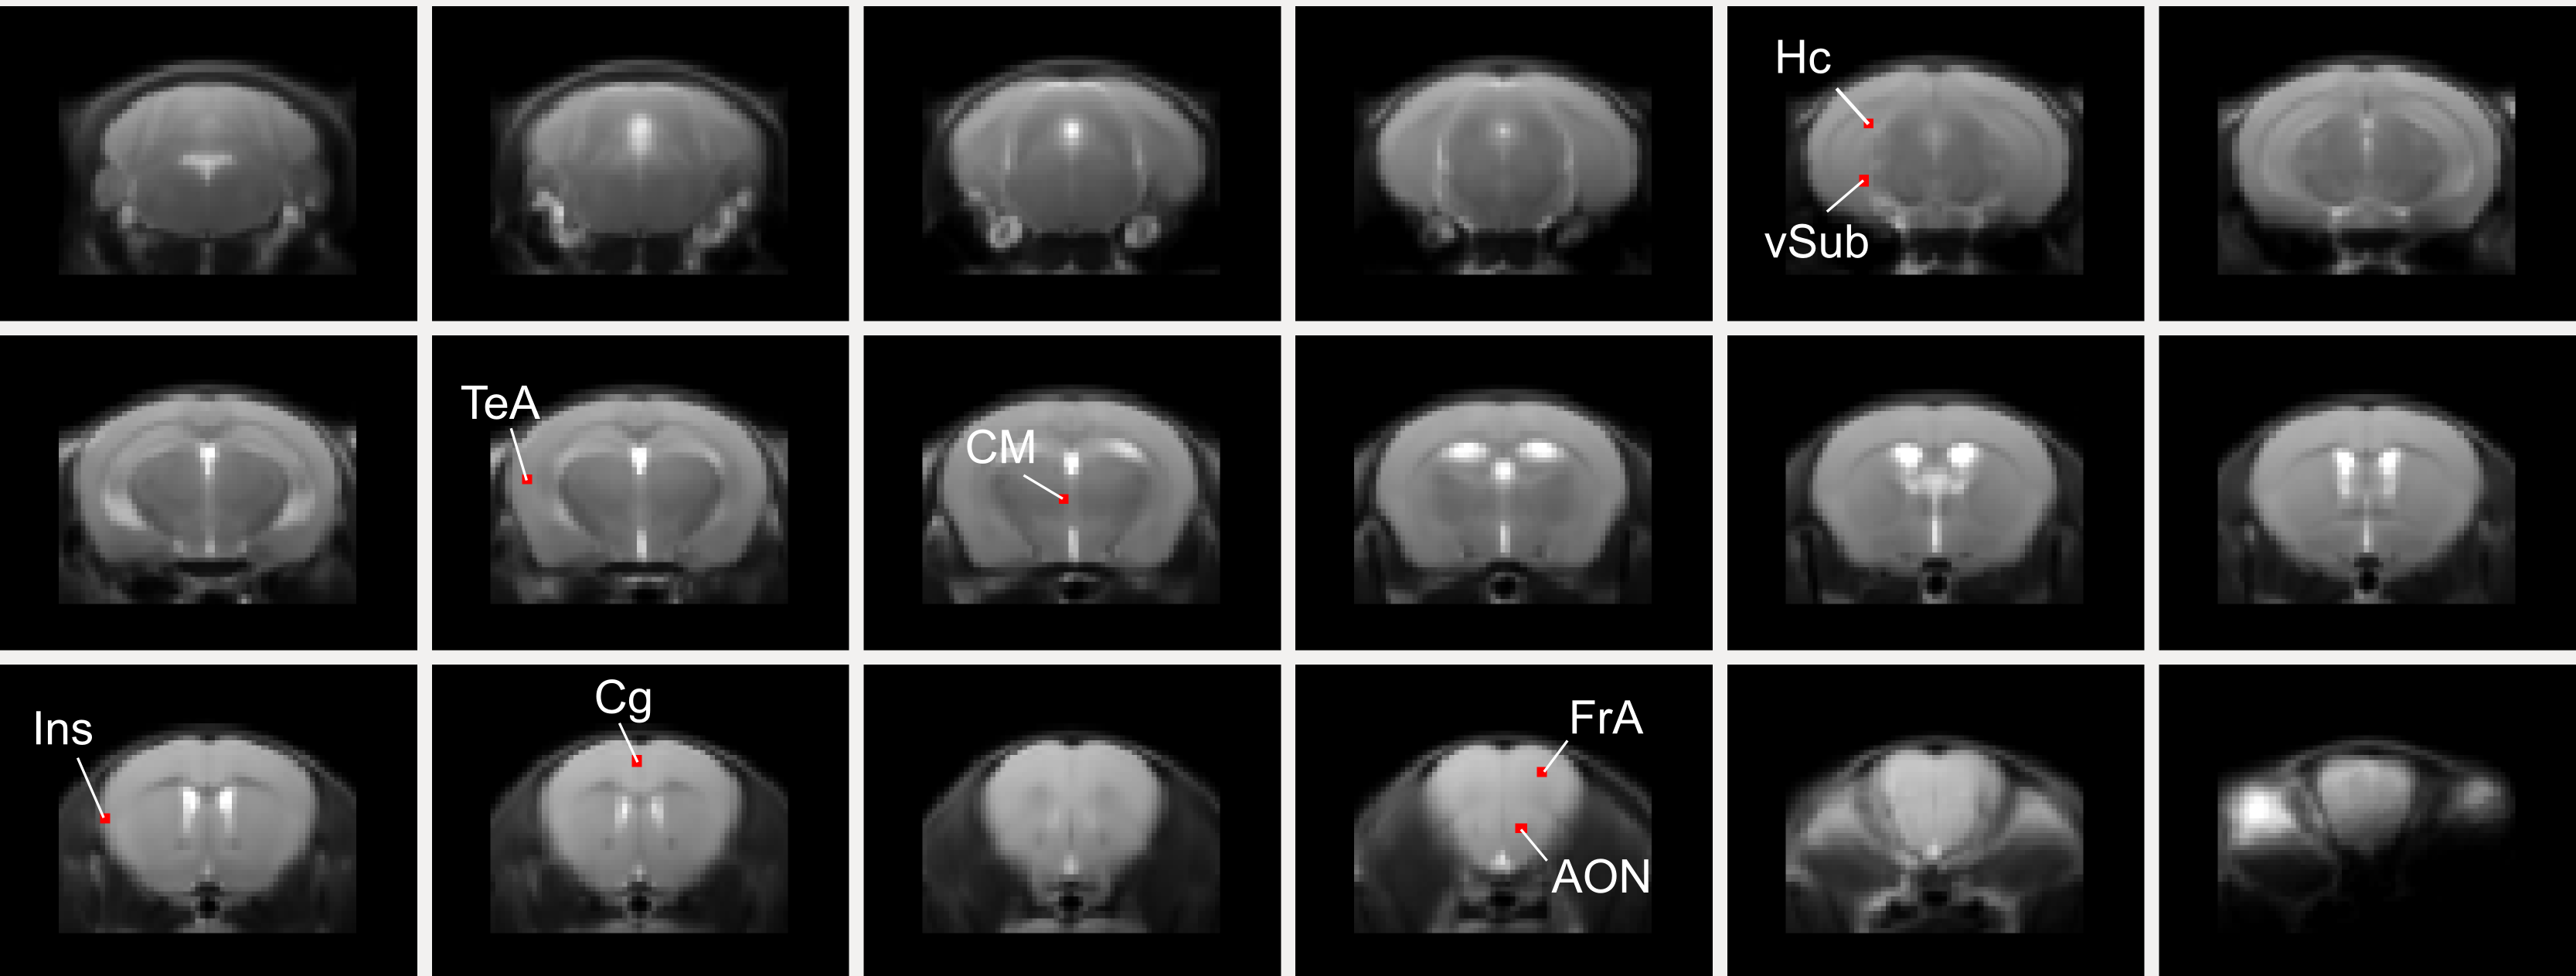
\includegraphics[scale=0.8]{figures/hubs_figure_s1_seed_locations_NEW.png}
    \decoRule
    \caption[Locations seeds used for inter-module hub connectivity
    analysis.]{Locations seeds used for inter-module hub connectivity analysis,
    each displaying the largest value of the network attribute in question for
    the given hub regions, overlaid on the anatomical template. }
    \label{fig:hubs_figs1_seed_location}
\end{figure}

\begin{figure}[th]
    \centering
    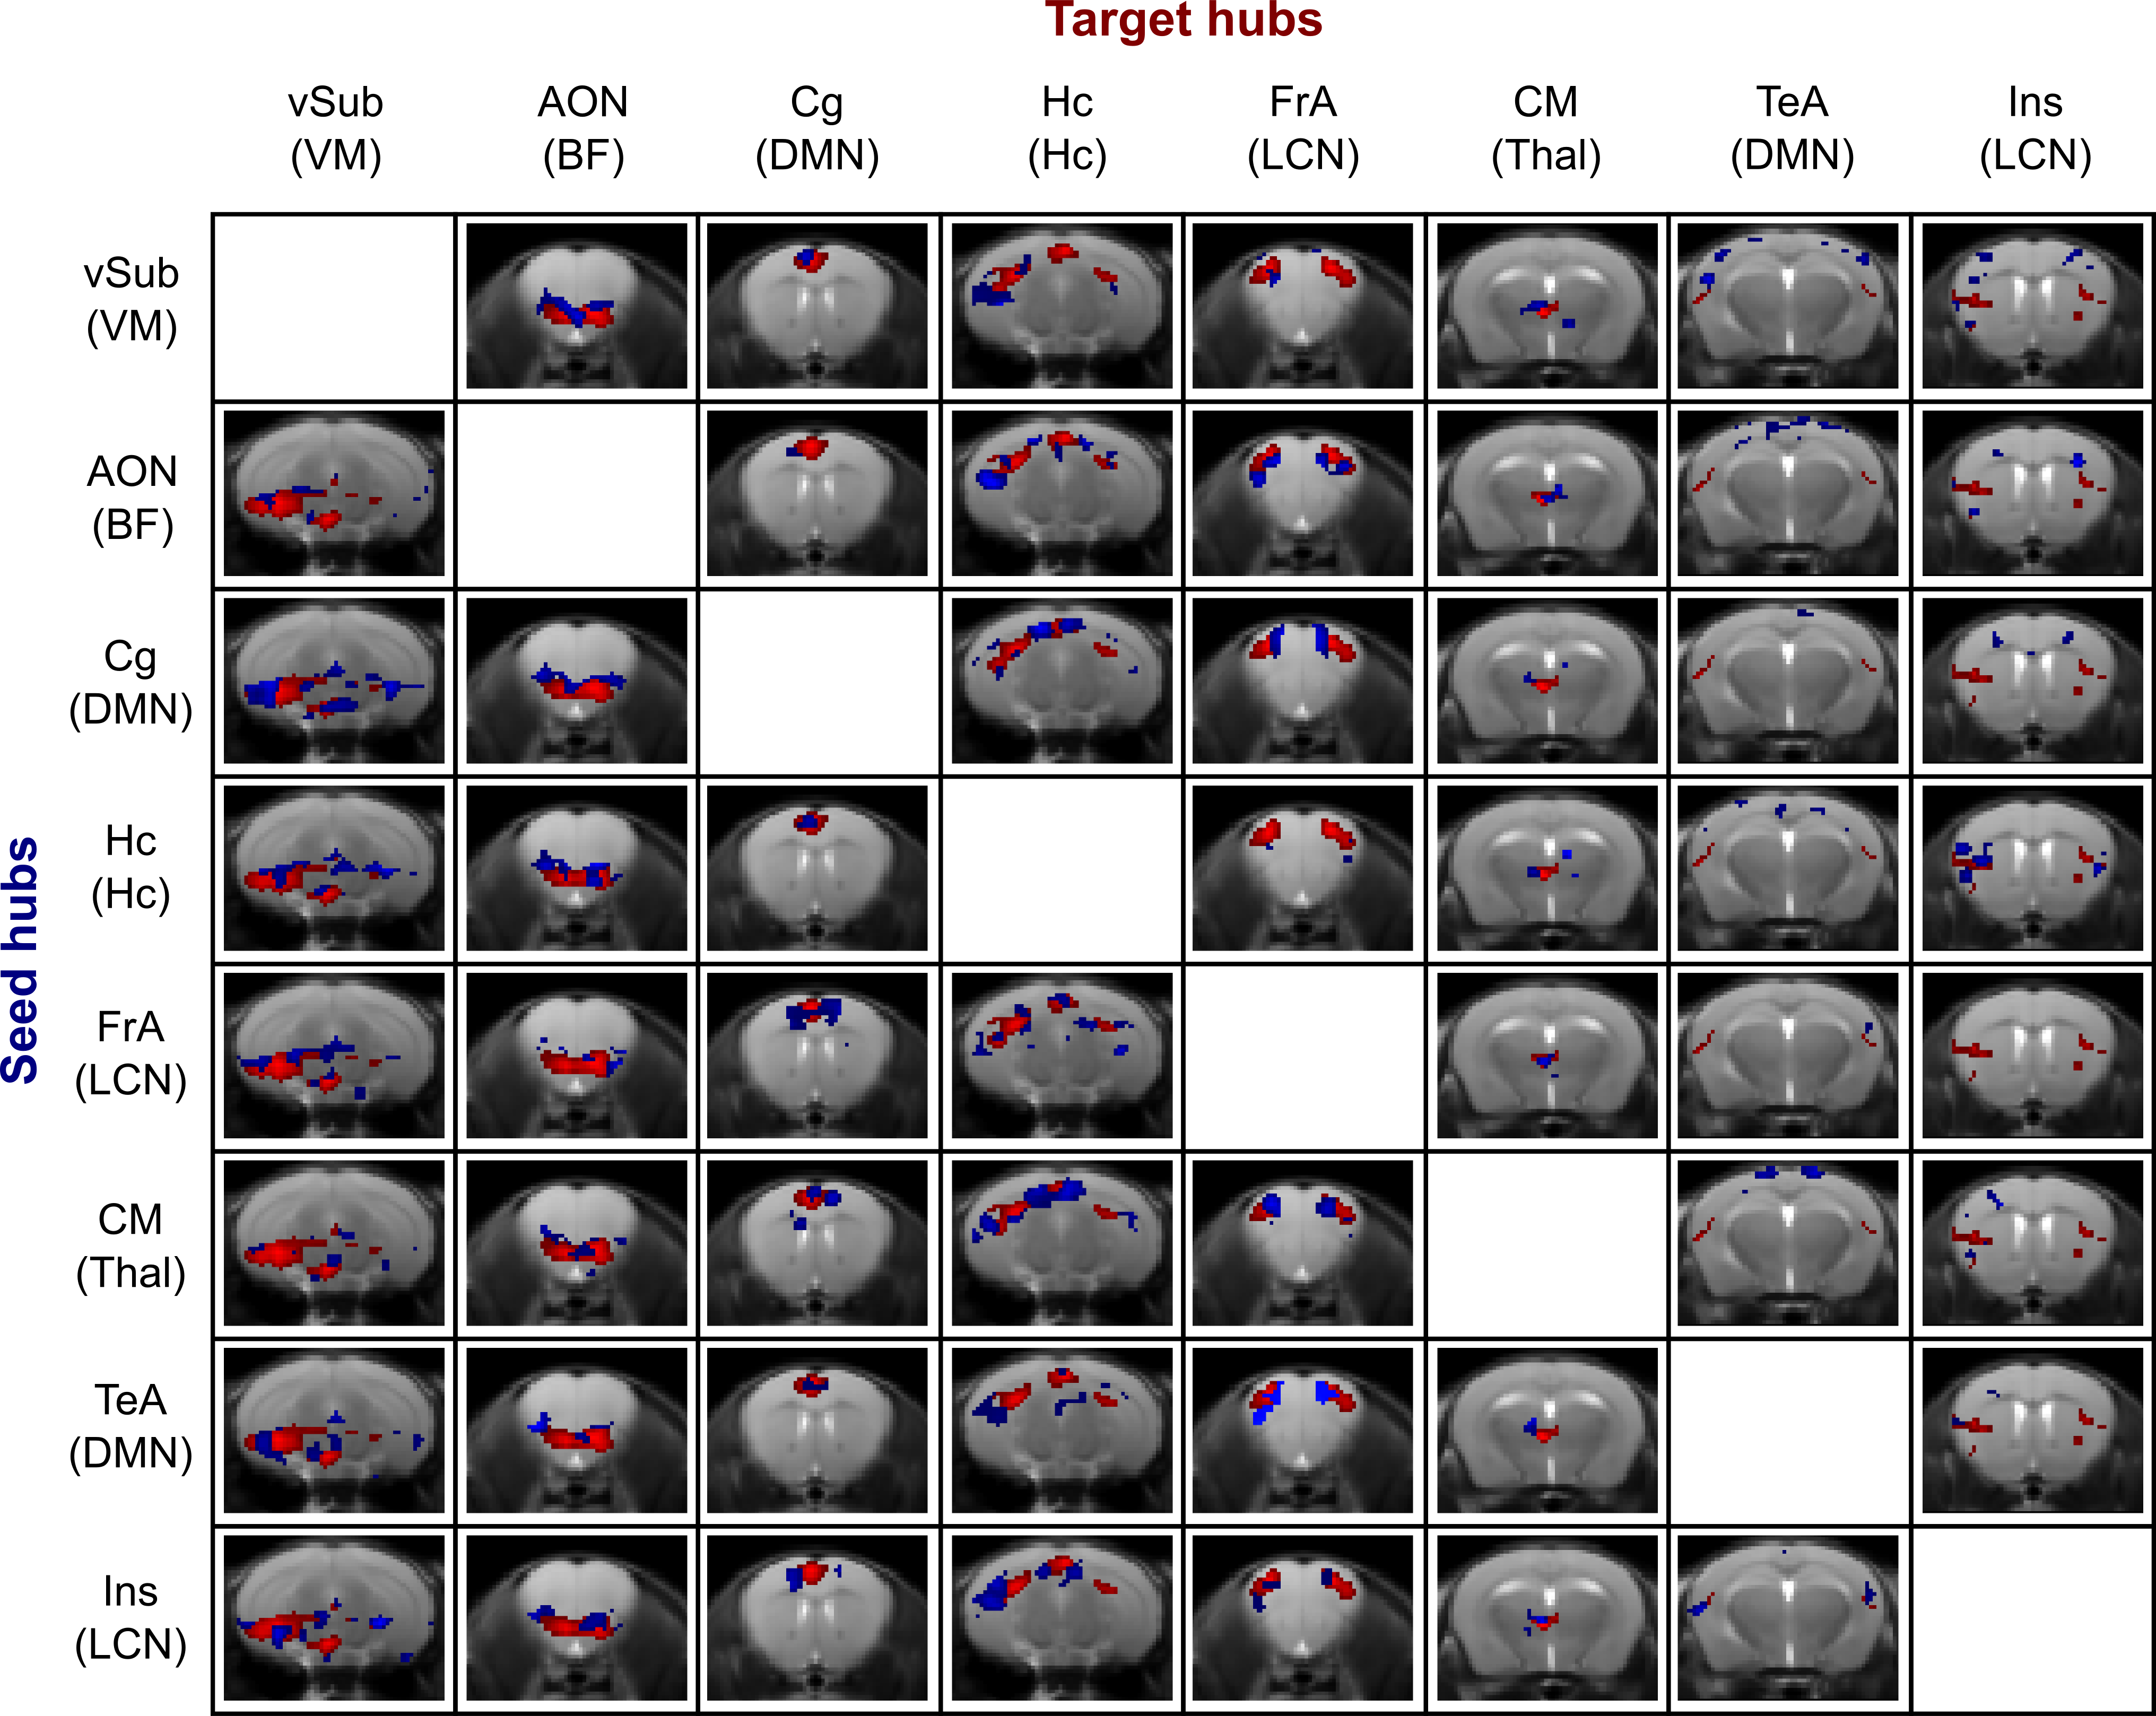
\includegraphics[scale=0.7]{figures/hubs_figure_05_voxel_overlap_NEW.png}
    \decoRule
    \caption[Functional hubs are mutually interlinked.]{Functional hubs are
    mutually interlinked. The strongest connections of each source hub to
    modules of target hubs (thresholded at 90th percentile for each module, in
    blue) are overlaid on top of target hub regions (in red). The results are
    shown on a representative coronal slice for each of the hub-module pair.}
    \label{fig:hubs_fig5_hub_connectivity}
\end{figure}

\begin{figure}[th]
    \centering
    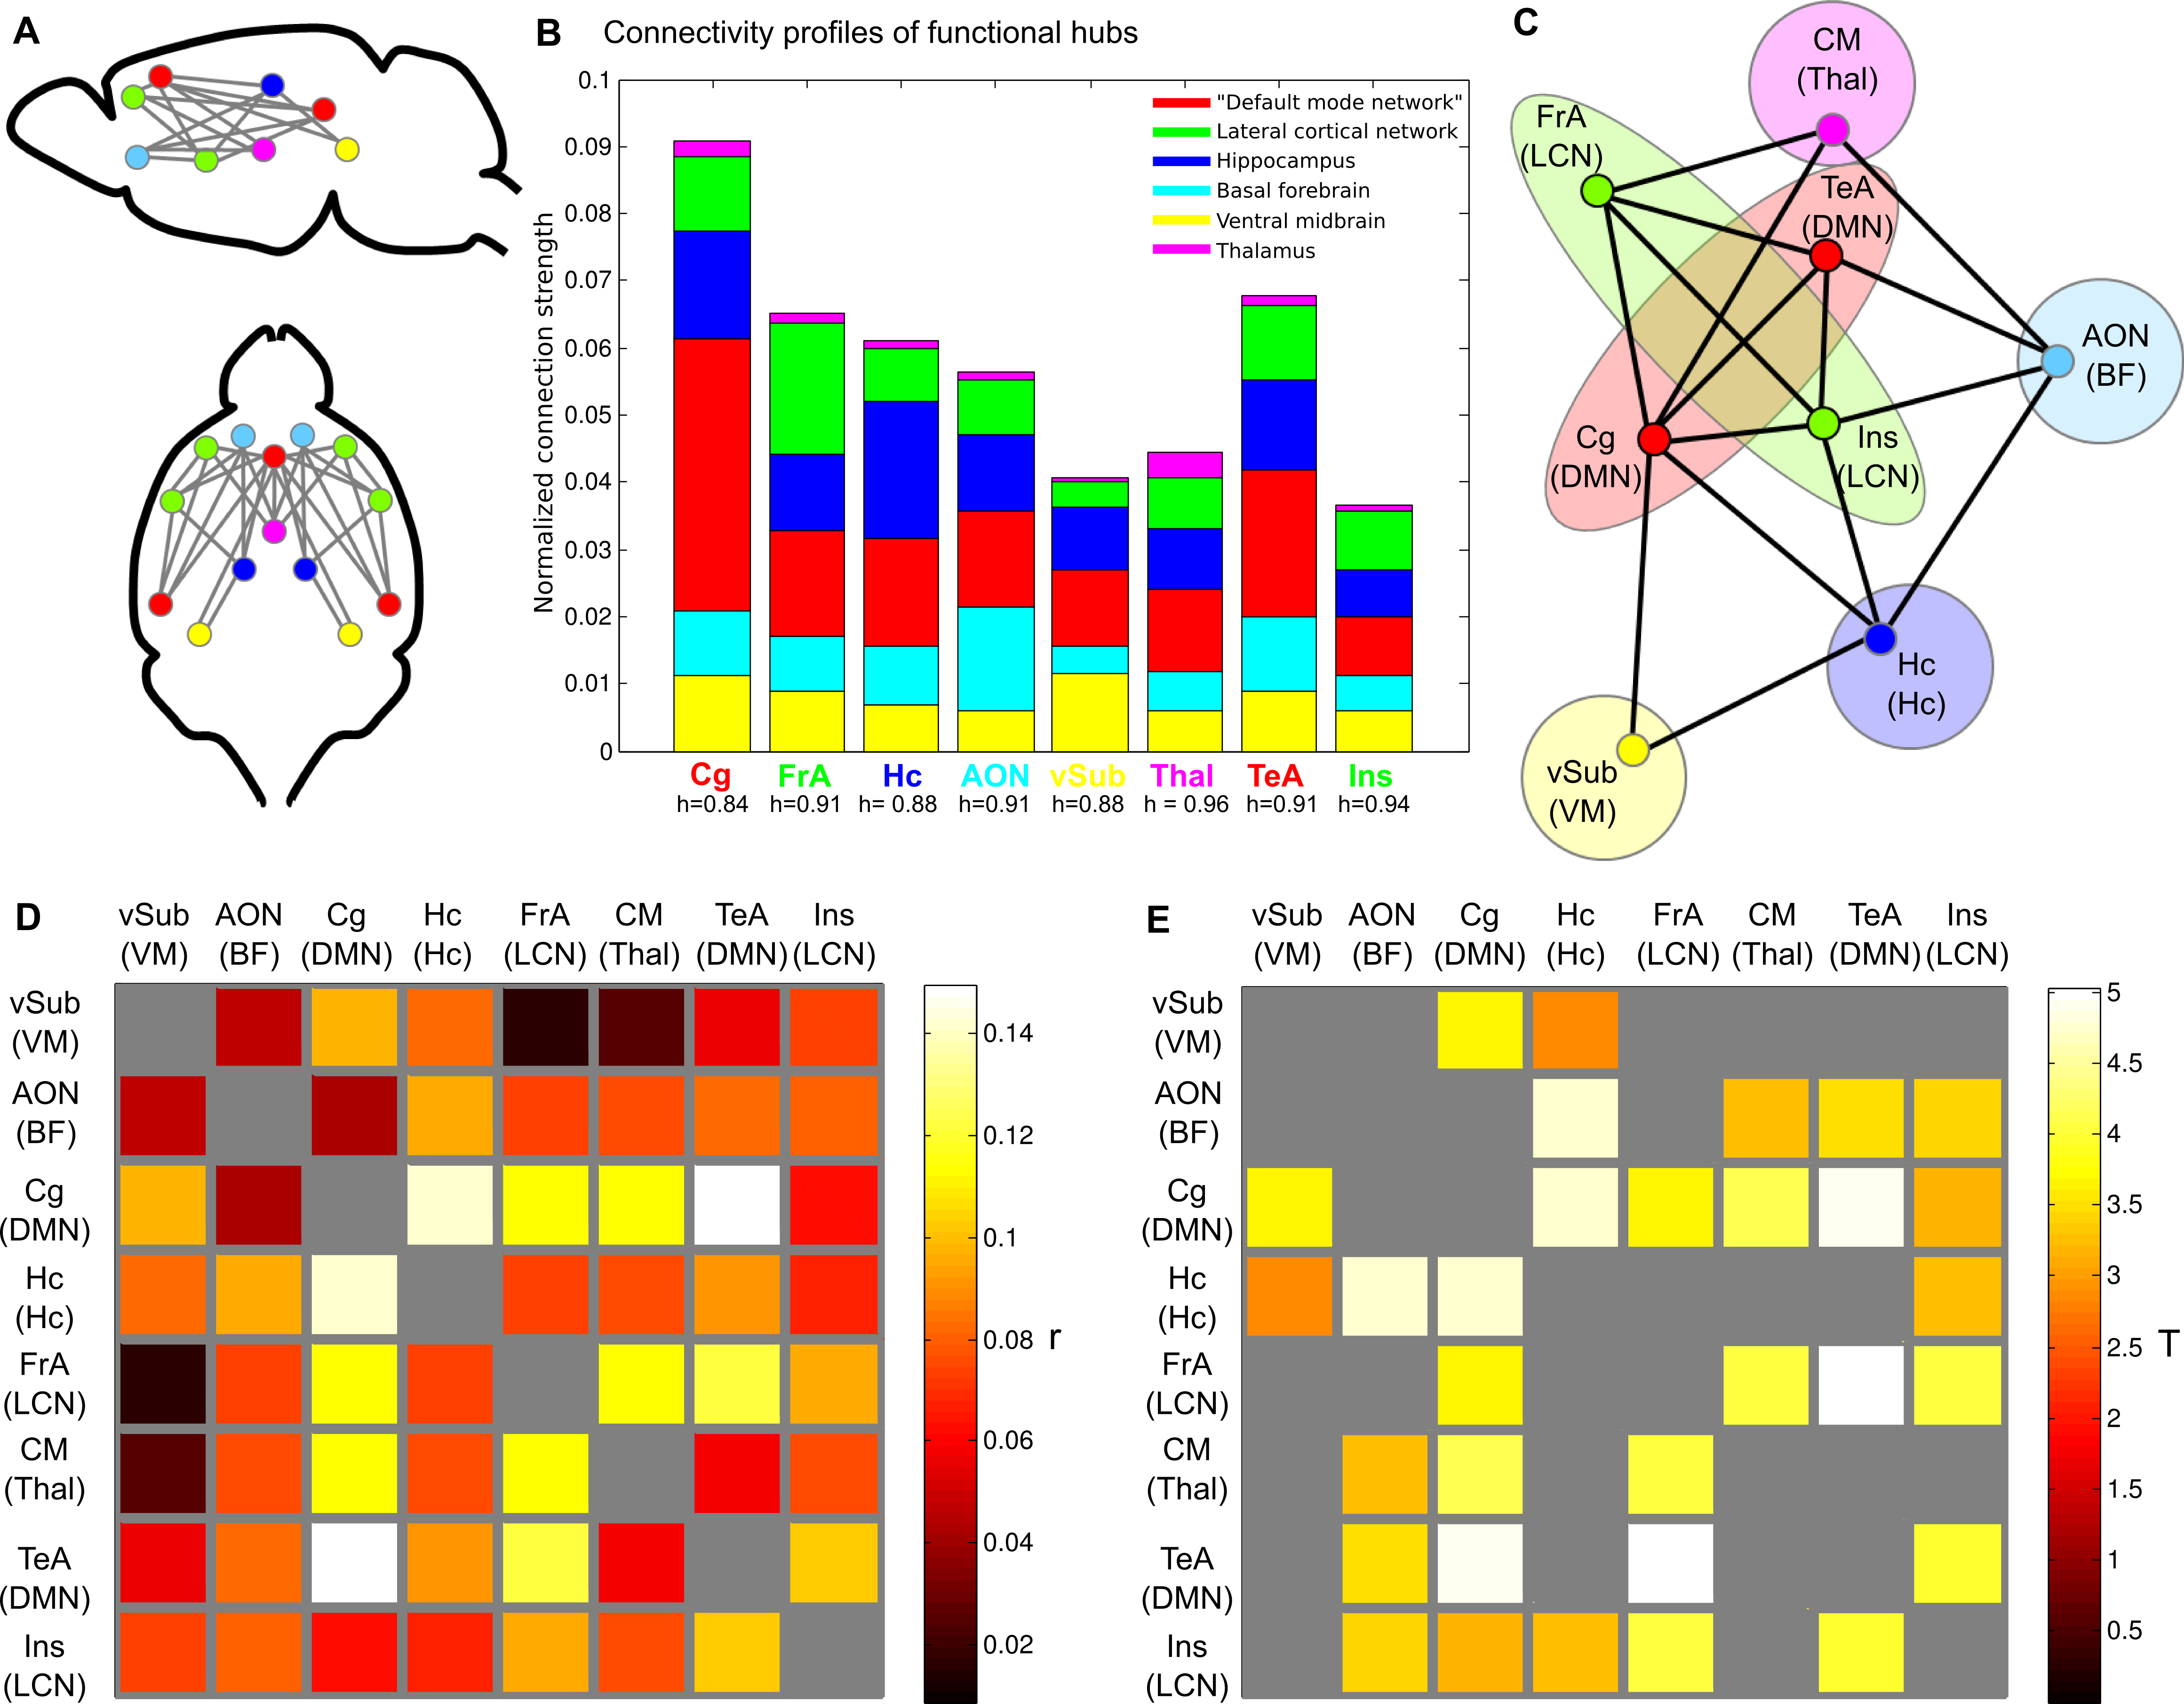
\includegraphics[scale=0.7]{figures/hubs_figure_06_hubs_connections_composite_NEW.png}
    \decoRule
    \caption[Connectivity relationships of candidate hubs.]{(\textbf{A})
    Approximate locations of candidate hubs of the mouse brain. Connections
    surviving statistical thresholding are indicated by a link between nodes
    (\textbf{B}) Connectivity profiles of candidate hubs, showing the proportion
    of their strength across all modules. (\textbf{C}) Graph representation of
    the connections surviving statistical thresholding, with node positions
    determined using the GEM algorithm. (\textbf{D}) Average correlation matrix
    for all pairs of identified hubs. (\textbf{E}) One sample t-tests for all
    pairs of identified hubs; non-significant connections (after FDR correction)
    are shown in grey.}
    \label{fig:hubs_fig6_hub_relationshiops}
\end{figure}


The interconnections between the eight candidate hubs were then characterised
directly to better elucidate the module connectivity that they subserve
(Fig.~\ref{fig:hubs_fig6_hub_relationshiops}). Many, but not all, of the hub
connections were significant, with the cingulate node (DMN module) having the
highest number of significant connections (6) to other candidate hubs, and the
temporal association cortex node (DMN) exhibiting the statistically strongest
connections, namely to the cingulate node (within-module) and to the frontal
association cortex node (across-modules, LCN). The ventral subiculum node (VM
module) had the least number (2) of significant connections to other candidate
hubs, to the cingulate cortex and hippocampal nodes (both across-modules, DMN
and Hc modules respectively).  Notably, both the DMN and LCN modules each
featured two putative cortical hubs, highlighting a key contribution of cortical
hubs within these circuits (i.e.  cingulate, temporal, frontal association, and
insular cortices) as prominent integrative nodes of rsfMRI connectivity networks
in the mouse brain. 

The connectional profiles of candidate hubs attest to the widespread
connectivity of hubs both within their own module and across the whole
functional network (Fig.~\ref{fig:hubs_fig6_hub_relationshiops}B).
Interestingly, a prominent integrative role of the DMN module was apparent, as
this region receives the largest share of the connection strength from all hubs
(excepting connections within a hub’s own module), although it is only second in
size to the ventral midbrain module.

\section{Discussion}

We have demonstrated the presence of distinct functional modules in the mouse
brain, and a set of anatomically localised, mutually interconnected candidate
hub regions acting as cross-module functional integrators. Our approach provides
a fine-grained description of the mouse functional connectome that can serve as
a reference and complement ongoing research in the meso- and large-scale
connectional architecture of this species \parencite{oh2014, stafford2014,
zingg2014}. It
also opens the way to targeted manipulations of hub nodes in mouse models of
brain pathology, a line of research that may advance our understanding of the
elusive role of functional hub regions in neuropsychiatric states
\parencite{vandenheuvel2013}. Importantly, we interrogated the mouse connectome at a
high, voxel-scale spatial resolution and worked with fully-connected,
fully-weighted networks, hence minimising bias induced by parcellation schemes
and issues associated with arbitrary thresholding and/or binarisation
\parencite{bullmore2009}.

Modular organization is central to functional segregation in the brain, whereby
distinct neuronal processing is performed by regions organized in functional
modules \parencite{sporns2013}. Studies of functional modular organization in the human
brain have consistently reported the presence of distinct distributed modules
corresponding to known functional brain systems, such as the default mode,
dorsal attention or somato-motor networks \parencite{meunier2009, power2011,
yeo2011}. In
keeping with this, the mouse brain functional networks identified here can be
reliably related to established large-scale neuro-functional and neuroanatomical
systems of the mammal brain. The detection of a DMN module using graph-based
approaches is in good agreement with the results of classic (ICA- and
seed-based) rsfMRI network mappings in the rodent brain \parencite{schwarz2013a,
schwarz2013, sforazzini2016, stafford2014} and underscores the pivotal role of
this integrative network across mammal brain evolution \parencite{lu2012}. Similarly, the
presence of a lateral cortical module is in agreement with recent
seed-correlation and ICA rsfMRI studies in mice and rats where the presence of a
similar DMN-anticorrelated systems has been described \parencite{schwarz2013a,
schwarz2013, sforazzini2016}, thus leading to the hypothesis that such a network
could be a precursor of lateralised “task-positive” executive modules present in
humans and primates \parencite{fox2005}. Importantly, the identification of
functionally-distinct antero-posterior distributed cortical module components is
in excellent agreement with recent cortical connectivity mapping obtained with
tracer injections in the mouse cortex. Indeed, by applying graph-based analyses
of tracer-based structural connectivity, \textcite{zingg2014} identified two
major neocortical clusters (i.e., somatic sensorimotor and medial
antero-posterior networks) that exhibit remarkable  neuroanatomical overlap
with our LCN and DMN modules. Similarly, the same authors also identified two
lateral integrative subnetworks in the cortex (anterior insular and posterior
temporal) that can be related to the high connection diversity cortical hub
nodes identified in the present work. Collectively, these findings corroborate
the emerging view that functional correlations in spontaneous brain activity
are constrained and guided by patterns of anatomical connectivity
\parencite{honey2009, sui2014}, a notion that has been more recently
demonstrated also for the mouse brain \parencite{stafford2014}. 

The correspondence between our cortical modules and analogous functional
networks of the human brain is of high translational relevance, as the approach
permits to identify key topological landmarks that can guide cross-species
extrapolation of neural circuit research in health and pathology. In this
respect, our work represents a significant advance over previous graph-based
attempts to unravel the rodent’s functional topology \parencite{bifone2010,
dsouza2014, liang2011, liang2012, schwarz2008, schwarz2009}. Indeed, while these
previous studies identified plausible functional modules, including large
cortical partitions \parencite{liang2011} and some subcortical networks similar
to those described here (e.g.  basal ganglia and hippocampus)
\parencite{dsouza2014, liang2011}, they did not to reveal antero-posterior
cortical networks like the rat’s DMN module, or the lateral cortical system, a
finding that could reflect discrepant experimental procedures as well as
heterogeneity in the regional parcellation schemes (coarse ICA-based or
anatomical volumes) and network thresholding strategies employed, or the fact
that the initial graph-based parcellation used cross-subject analyses of
responses to pharmacological stimuli \parencite{bifone2010, schwarz2008,
schwarz2009}. Likewise, the results of a recent attempt to map functional
modules and hubs in the mouse employing ICA-based functional parcellation
\parencite{mechling2014} resulted in a coarse modular organization that includes
some of the modules identified in this study (e.g. basal ganglia and
hippocampus), as well as a combination of cortical and subcortical structures
encompassing multiple neurofunctional systems of the brain (e.g. sensory motor
and limbic areas), which corroborate the underlying modular structure of the
mouse brain, but cannot be directly related to analogous functional modules of
the human brain.  The identification of neuro-biologically interpretable
functional modules is also key to the identification of candidate hub regions
deemed to link and integrate specialized functional systems
\parencite{sporns2013}. Using graph-based methods, numerous studies in humans
have converged on a limited set of regions that occupy a central position in the
functional topology of the human brain. These regions include anterior and
posterior cingulate cortices, the insular cortex, and portions of superior
frontal cortex, temporal cortex and lateral parietal cortex \parencite{cole2010,
sporns2014, tomasi2011, vandenheuvel2013}. Importantly, the very same regions
have also been shown to be implicated in the anatomy of various brain disorders,
such as schizophrenia and Alzheimer’s disease, which can be investigated and
modelled in the mouse \parencite{buckner2009, crossley2014}. Consistent with
human findings \parencite{cole2010}, we identified high strength nodes in the
mouse brain located in midline regions within the DMN module, with a predominant
involvement of integrative areas such as the prefrontal, anterior and posterior
cingulate cortex. Notably, a striking neuroanatomical correspondence also exists
between our high connection strength hubs, and high degree structural
connectivity hubs of the mouse based axonal tracing \parencite{stafford2014}, a
finding that recapitulates a fundamental neuro-architectural feature of the
human brain \parencite{vandenheuvel2013}. Similarly, high connection
diversity regions were identified in the temporal association cortex and, albeit
with a lower degree of statistical confidence, also in the anterior insula, two
areas classically implicated in multimodal integration \parencite{gogolla2014}.
Furthermore, the same areas have been recently described in the human brain as
regions of high participation coefficient, a binary network counterpart to
connection diversity \parencite{power2013}. Importantly, most of the hub regions
we identified in the mouse brain exhibit robust and specific mutual
inter-connections, a finding which is consistent with an integrative functional
role of these nodes, and which argues against a predominant confounding
contribution of the correlational nature of rsfMRI-based networks
\parencite{power2013}.  Collectively, these correspondences underscore the
translational relevance of our findings, and support the notion that the mouse
brain contains evolutionary-conserved cortical foci serving as integrators of
segregated systems in the mammal brain.

The fact that our experiments were performed in anaesthetized animals raises the
question as to the degree to which the observed effects reflect the functional
architecture of the mouse brain in conscious states. Two recent mouse rsfMRI
studies have highlighted different connectivity signatures and reduced
inter-hemispheric connectivity as a function of anaesthetic regimen
\parencite{grandjean2014, jonckers2014}. The present work was performed in
halothane-anaesthetised animals, a regimen that appears to be particularly
suited to map distributed rsfMRI circuits in this species for several reasons.
First, halothane ensures motion control and stable hypnosis while preserving
cerebral blood flow autoregulation \parencite{gozzi2007} and cortical electrical
responsiveness \parencite{orth2006} without the occurrence of burst suppression
activity, a phenomenon associated with significant rsFC alterations
\parencite{liu2011}.
Consistent with this, our recent work \parencite{sforazzini2014, sforazzini2016,
zhan2014} demonstrates the presence of (1) robust homotopic inter-hemispheric
functional connectivity in both cortical and subcortical areas, and (2)
distributed networks remarkably similar to those seen in conscious (and lightly
anesthetised) rats and primates, anatomically homologous to the human salience
network (SN) and default-mode network (DMN) \parencite{hutchison2010, lu2012,
rilling2007, schwarz2013, schwarz2012, vincent2007}. Importantly, the
observation of a DMN-like network in the mouse has been recently replicated by
an independent group \parencite{stafford2014} using a different anaesthetic
(isoflurane), a finding that corroborates a neurobiological foundations of this
cortical module. Moreover, BOLD fMRI oscillations in the DMN-like network
exhibit anti-correlations with neighbouring fronto-parietal areas, a cardinal
feature of the human and primate DMN \parencite{fox2005}. By showing analogous
networks using cerebral blood volume weighted signals, we also demonstrated that
these spontaneous fluctuations are not significantly contaminated by large blood
vessels \parencite{sforazzini2016}. Finally, we recently demonstrated excellent
spatial correspondence between rsfMRI signals obtained during light anaesthesia
and electrophysiological coherence signals in freely-behaving animals,
suggesting that the anaesthetic protocol negligibly influences intrinsic rsfMRI
connectivity profiles \parencite{zhan2014}. Collectively, the identified rsfMRI
networks exhibit significant correspondence with analogous measurements in awake
habituated rats and human studies, thus legitimating the extrapolation of our
results to conscious states. Consistent with this notion, global topological
features of rsfMRI networks were found to be well maintained in the anesthetized
rat brain when compared to awake (restrained) states, despite the use of much
higher (2.25-fold) minimal alveolar concentration levels of anaesthetic than the
present work \parencite{eger2003, liang2012, sonner2000}. The remarkable overlap
between modules and hubs identified in this work and recent tract tracing
mapping in the mouse \parencite{zingg2014}, as well as analogous graph-based
mappings in conscious human brain provide further empirical support to a
marginal confounding contribution of anaesthesia to our findings.  

\section{Conclusion}

In conclusion, our results describe topologically distinct neuro-functional
modules of the mouse brain, including a DMN-like module, and identify a set of
mutually-interconnected functional hubs that include well-characterised
integrative cortical structures. These findings reveal the presence of
evolutionarily conserved functional modules and integrative hubs in the mouse
brain, and support the use of this species to investigate the elusive
neurobiological underpinnings of the functional hub aberrations described for
several pathological states. Importantly, our approach also provides a
fine-grained description of the mouse functional connectome that complements and
integrates ongoing research in the large-scale connectional architecture of this
species. 
